
\title{QBUS3830\\ Advanced Analytics\\ Team Project}
\author{Yiran Jing \\ Rhys Kilian \\Harry Nicol
}
\date{November, 2018}
\documentclass[11pt]{article}
\usepackage[toc,page]{appendix}
\usepackage{graphicx} 
\usepackage{float}
\usepackage{caption}
\usepackage{subcaption}
\usepackage{geometry}
\usepackage{amsmath}
\usepackage{lscape}
\usepackage{natbib}
\usepackage{adjustbox}
\usepackage{changepage}
\usepackage{multicol}
\usepackage{booktabs}
\geometry{
	a4paper,
	total={170mm,257mm},
	left=15mm,
	right=15mm,
	top=20mm,
	bottom=20mm}

\newcommand{\HRule}[1]{\rule{\linewidth}{#1}}
\setcounter{tocdepth}{5}
\setcounter{secnumdepth}{5}

\begin{document}

\title{ \normalsize \textsc{QBUS3830: Advanced Analytics}
		\\ [2.0cm]
		\HRule{0.5pt} \\
		\LARGE \textbf{\uppercase{Reducing Power Supply Costs in South Australia using Time-Series and Machine Learning Methods}}
		\HRule{2pt} \\ [0.5cm]
		\normalsize \vspace*{5\baselineskip}}
\date{November, 2018}
\author{Yiran Jing 460244129\\ Rhys Kilian 440246200\\Harry Nicol 450383867\\}
\maketitle

\pagenumbering{gobble}
\newpage
\thispagestyle{empty}
\section*{Executive Summary}

Our neural network model forecast for South Australian power demand was able to outperform the industry standard model by 11.12\%. This project used very short-term load forecasting methods to improve the one step ahead (30 minute) demand forecast for the state of South Australia. In order to reach this optimal model we added Bureau of Meteorology Adelaide weather data as an additional variable on top of variables from the energy market operator. Using the 30 minute time series data for the input variables price, demand and temperature we considered traditional time series models, machine learning methods and benchmark models. 
\\
\\
Through EDA we identified a strong daily and weekly pattern for demand which was utilised in auto regressive models and linear models. During feature engineering we created dummy variables for blackouts, heatwaves and season. The optimal neural network was identified through a randomised grid search cross validation of hyperparameters. Combination forecasts were considered but could not beat the performance of the neural network model. The expansion of input variables to include weather variables allows our neural network to be so successful that it could save millions of dollars for energy providers. By creating more accurate demand forecasts there will be less supply induced blackouts in South Australia allowing for a more reliable and less costly energy market.

\addcontentsline{toc}{section}{Executive Summary}
\newpage
\tableofcontents
\newpage
\setcounter{page}{1}
\section{Introduction and Business Context}
\pagenumbering{arabic}

The South Australian energy market has undergone a variety of challenges in recent years including extreme weather events, debate over its reliance on renewable energy and a series of power outages. 
\\
\\
The Australian Energy Market Operator (AEMO) provides historical energy demand and price data which is used by regulators and suppliers to predict the energy demand 30 minutes in to the future, known as very short-term load forecasting (VSTLF). Our project seeks to improve the accuracy of VSTLF and ensure that shortfalls in supply occur less frequently to improve the costs of energy for consumers and providers. The industry standard loss function is the mean absolute percentage error (MAPE). It has been estimated that a reduction of 1\% MAPE would lead to a US\$1.6 million saving per year for a 10-gigawatt generator \citep{hobbs_analysis_1999}. 
\\
\\
South Australia's capital city Adelaide is subject to some of the most extreme temperatures of any state in Australia. It is the driest capital city (Mack, 2013) and has a reputation for its "blistering heatwaves". These extreme weather events have put significant pressures on the state energy infrastructure (Saddler, 2013). The primary use for power is for heating and cooling (40\%) houses. The secondary driver for residential energy consumption is water heating. Hence our hypothesis is that changes in temperature are a good predictor for energy use. 
\\
\\
By combining historical climate, energy demand and price we aim to improve the MAPE of current industry models to provide cost savings to regulators and energy providers. 

\section{Data Understanding}
\label{section: data_processing}
Our model uses data sourced from AEMO \citep{noauthor_data_2018} and the Bureau of Meteorology \citep{noauthor_historical_2017}.\\ The key variables from the AEMO data were:
\begin{enumerate}
\item \textbf{Time:} The time variable was available in 30 minute intervals from 1998 to 2018. 
\item \textbf{Price:} The variable `price' is an average of the dispatch prices in South Australia over each half hour period and is known as the spot price. Industry prediction models use the spot price instead of the dispatch price because it is extremely volatile in 5 minute intervals. Predicting 30 minutes ahead is more useful for adjusting energy supply. It's units are Australian dollars. 
\item \textbf{Demand:} Demand is measured in megawatts (MW) for the entire state of South Australia.
\end{enumerate}


\noindent The key variables from the BOM data were:
\begin{enumerate}
\item \textbf{Time:} This variable was in 1h intervals for the period  01/05/2016 - 30/04/2017.
\item \textbf{Station number:} This identifies which weather station the measurements comes from
\item \textbf{Value:} For each time period there were 4  different observations within the same variable `value'.
\begin{enumerate}
\item Current temperature (Celsius). 
\item Maximum temperature in that period (Celsius).
\item Minimum temperature in that period (Celsius).
\item Amount of rain in that period (mm).
\end{enumerate}
\end{enumerate}
    

\section{Data Processing}

\subsection{Time Period} 
A year of data  was extracted  from the AEMO and the BOM between 1/05/2016 to 30/04/2017. This period was selected as it contains the summer where three significant heat waves occurred. Furthermore, the more recent weather data is extremely dirty (filled with missing values and wrong records). We considered the benefits of using complete data outweighed the benefits of using the most recent data. Hence in order to give our model the best chance of improving the industry standard we chose to focus on this period. 
 
\subsection{Weather station} 
The BOM has a large selection of weather stations to select from. We selected the Adelaide Airport weather station as it is considered the most reliable being located at an major airport. Furthermore the weather in Adelaide is most likely to effect the power consumption of South Australia as the capital has the highest population density. Adelaide contains over 75\% of South Australia's population (ABS, 2018).

\subsection{Missing data} 
In the weather data on the 31/05/2016 there was missing data points for 12am, 1am, 2am, 3am and 4am. This missing data was linearly interpolated. 

\subsection{Duplicate values} 
At 2pm each day the BOM data had double the amount of observations then at every other period. We concluded that this is due to the method of processing of the data. Hence we dropped the second set of values at 2pm each day.

\subsection{Filtering weather data of interest}
Of the four weather variables we selected current air temperature as the most relevant for our model. We excluded rainfall as this has no strong evidence for correlation with energy demand unlike temperature. In order to prevent multicollinearity issues we had to choose one of the three temperature variables. We selected current air temperature.

\subsection{Matching time interval between data sources} 
BOM weather data intervals needed to be matched to the time intervals of AEMO data 30 minute intervals. The hourly data was expanded to 30 minute intervals via linear interpolation.

\section{Exploratory Data Analysis}
Our aim is to produce a prediction for the explanatory dependent variable, power demand, using the regression variables price and temperature.
\subsection{Non-parametric regression}

After plotting the values for air temperature and price against their index's it is clear that nonlinear time series relationship is true for both variables. This suggests that a non-linear model is likely going to perform better with this data.

\begin{figure}[H]
\centering
\begin{minipage}{.6\textwidth}
  \centering
  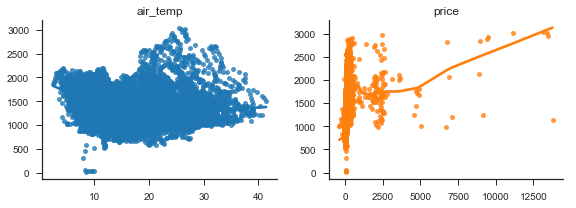
\includegraphics[width=0.95\linewidth]{EDA_temp_price.png}
   \caption{Local linear regression for variables air temperature and price}
   \label{fig:EDA_temp_price}
\end{minipage}%
\end{figure}

\subsection{Time-Series Decomposition}
\label{section:time_series_decomposition}

Time series is a function of 4 components: trend component or the systematic long term trend; seasonal component which is the regular fixed period fluctuations; cyclic components representing fluctuations in the series that are not of fixed period (e.g. business cycle); and residual which is the irregular or error component. The results for this decomposition are shown in Figure \ref{fig:demand_before} in Appendix \ref{appendix:further_eda}. 
\\
%\subsubsection{Outcomes of decomposition}

\noindent The time-series decomposition plot highlights a clear seasonal variation in each variable which is not proportional to the trend component. Hence, we elect to use the additive model for decomposition. Additionally, there are two clear outliers in the price variable.
Further investigation found that these points occur on the 20/03/17 between 13.00-14.00 and the 21/03/17 between 11.00-13.00. During these periods the price was recorded at extreme levels from \$929-\$2651/MW, caused by an outage in Victoria.
\\
% The AEMO is obliged to publish reports when there are extreme power prices. 
% In this case there was a planned network outage in Victoria along one of the key connection points to South Australia. This meant that South Australia was only connected to the national energy market via one connection point. In order to plan for the situation where this single remaining line was cut AEMO artificially increased the demand to 35MW. This meant that energy providers bids were as high as \$9000/MW in order to meet this 35MW requirement. The spike in price ended when the Victorian outage ended and the spare 35MW was no longer required.

%As the extreme prices during this period were a product of artificial market forces it is reasonable to remove these points.
%\subsubsection{Remove outliers}
\noindent In order to improve our modelling we decide to place a cap of \$400MW as the maximum price not considered an outlier. This was determined by considering the normal maximum price in the energy market. The outliers made up less than 1.4\% of total data which we decided was reasonable. Similarly we capped demand at 1900 MW which effects less than 5\% of the data. The time series decompositions before and after this cleaning are shown in the appendix (Figures \ref{fig:price_before} - \ref{fig:demand_after}).

\subsection{Complex seasonality}

With high frequency data it is common to observe multiple seasonal patterns. Complex seasonal analysis allows for identification of patterns with a non-integer period \citep{de_livera_forecasting_2011}. From our analysis on the demand cycle we observed a strong daily (seasonal 48) pattern and also a weekly (seasonal 336) pattern. The weekly seasonal pattern is stronger than the daily seasonal pattern. These patterns were identified using a a Box-Cox transformation of the demand data and complexity plot, as per Figure \ref{fig:complex_demand}.
\\


\begin{figure}[htpb!]
\centering
\begin{minipage}{.6\textwidth}
  \centering
  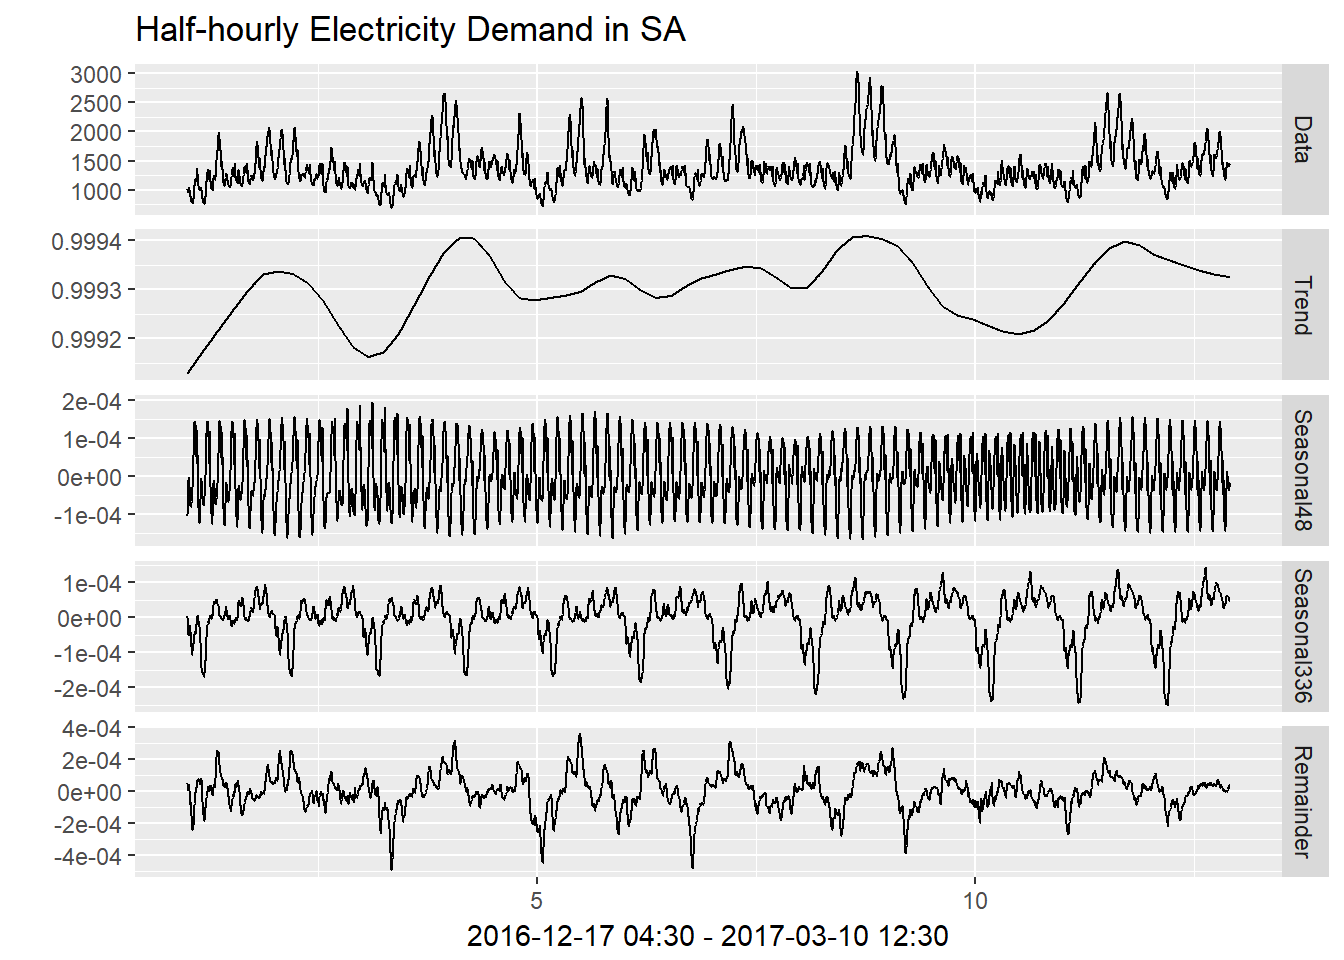
\includegraphics[width=0.95\linewidth]{complex_demand.png}
   \caption{Complex seasonality plot for demand}
   \label{fig:complex_demand}
\end{minipage}%
\end{figure}

\noindent However, there are some limitations of this complex seasonality analysis. Firstly these models only allow for regular seasonality. They are unable to capture seasonality associated with moving events such as Easter. Furthermore, they only show patterns the patterns present in the data. In this case we didn't provide enough data for it to show an annual pattern. At the other extreme it also struggles to capture sub daily patterns. These are likely included in the daily and weekly pattern that the above figure has identified.

\section{Feature engineering}

Extensive feature engineering was carried out in the project, for several reasons. Firstly, the machine learning models, including the linear and neural network models, required predictors in order to model the the response variable, South Australian power demand. In the past, this has been done by completing an autocorrelation analysis, as demonstrated by \citet{sood_electricity_2010}, and then using the relevant lagged demand data as a predictor. This process is outlined in Section \ref{section:lags}. Furthermore, the inclusion of several dummy variables, to model blackouts and heatwaves for example, was used to improve the model performance. The inclusion of these additional variables to predict electricity demand is not well documented and has been highlighted as an area for future work \citep{kotillova_statistical_2012}. Hence, this report aims to analyse the effects of these engineered predictors, which are outlined in this section of the report.

% \subsection{Clean data}
% % need justify reason, and might give comparation plots result before and after (plot can in appendix, but mention here)
% % clean price and demand,(plot and reason all in notebook)

% The data was cleaned using the techniques outlined in Section \ref{section:time_series_decomposition}.

\subsection{Dummy variables}
\label{section:dummy_variables}
In the study of econometrics, it is common to include dummy variables in models to improve the performance of time-series methods. For instance, \citet{moller_econometric_2015} made use of a number of dummy variables, model electricity demand in Denmark, from an econometrics perspective. In this investigation, dummy variables were created for: blackouts, heatwaves, seasons and public holidays. All with the purpose of increasing predictive performance, particularly for the machine learning models. 

\subsubsection{Blackouts}
\label{section:blackouts}

During the period over which the demand data was collected, there were several blackout events which affected the power demand during this period. The term blackout refers to the phenomena when power distribution is either bottlenecked or completely stopped, due to an invent such as a storm or a transmission fault. They are characterised by sudden decreases in demand, immediately followed by a large spike when distribution is brought online. Therefore, it was deemed critical to model these events with the use of a dummy variable. The blackout events within this dataset were defined by AMEO \citep{noauthor_sa_2016}:

\begin{enumerate}
\item \textbf{28th September, 2016} - a storm cutting the power to 1.7 million residents of South Australia until 10:00pm 
\item \textbf{27th December, 2016} - blackout due to storm damage
\item \textbf{8th February, 2017} - excess load shedding during a heatwave
\end{enumerate}

\noindent These events were modelled as per Equation (\ref{eqn:dummy_blackout}).

\begin{equation}
\label{eqn:dummy_blackout}
dummy\_Blackout = 
  \begin{cases}
	1 & \text{if blackout during time period} \\
    0 & \text{otherwise}
  \end{cases}
\end{equation}

\subsubsection{Heatwaves}
\label{section:heatwaves}
Heatwaves were also important events to capture using dummy variables. Our research indicated that a large component of South Australia's power demand is cooling, which is related to heatwave events \citep{griffiths_heatwave_2018}. It was expected that heatwaves would cause large upward spikes in demand, and therefore, to ensure the accuracy of predictive models, was required to be included as a predictor. The heatwaves in this dataset included:

\begin{enumerate}
\item \textbf{9-14th January, 2017} - temperatures exceeding 48 degrees
\item \textbf{17-21st January, 2017}
\item \textbf{31st January, 2016 -   12th February, 2017}
\end{enumerate}

\noindent These were feature engineered as per Equation (\ref{eqn:dummy_heatwave}).

\begin{equation}
\label{eqn:dummy_heatwave}
dummy\_Heatwave = 
  \begin{cases}
	1 & \text{if heatwave during time period} \\
    0 & \text{otherwise}
  \end{cases}
\end{equation}

% \subsubsection{Public Holidays}

% There is evidence that energy consumption is lowest on holidays. For instance, South Australia Christmas Day had the least amount of energy used in the whole of 2012 \citep{saddler_past_2013}. This pattern has been shown to occur similarly for other public holidays suggesting a positive relationship between economic activity (i.e. business working days) and power consumption in South Australia. This pattern has also been previously observed on the weekends too \citep{saddler_past_2013}. Therefore, the drop in demand, caused by no-working days, was included as a predictor using Equation (\ref{eqn:dummy_holiday}).
% \begin{equation}
% \label{eqn:dummy_holiday}
% dummy\_Holiday = 
%   \begin{cases}
% 	1 & \text{if holiday during time period} \\
%     0 & \text{otherwise}
%   \end{cases}
% \end{equation}

\subsubsection{Season}
\label{section:season}
Given that the season affects the temperature the rationale for including dummy variables for the seasons follows on from Section \ref{section:heatwaves}. It is expected that in Summer the power demand would be high due to cooling devices being used. Alternatively, we expect the power demand to be high in Winter as heaters will be used. Hence, to model the four seasons, three dummy variables, as per Equations (\ref{eqn:dummy_Summer})-(\ref{eqn:dummy_Spring}) were used to prevent any issues with multicollinearity (where Autumn is the reference season). 

\begin{equation}
\label{eqn:dummy_Summer}
dummy\_Summer = 
  \begin{cases}
	1 & \text{if Summer during time period} \\
    0 & \text{otherwise}
  \end{cases}
\end{equation}

\begin{equation}
\label{eqn:dummy_Winter}
dummy\_Winter = 
  \begin{cases}
	1 & \text{if Winter during time period} \\
    0 & \text{otherwise}
  \end{cases}
\end{equation}

\begin{equation}
\label{eqn:dummy_Spring}
dummy\_Spring = 
  \begin{cases}
	1 & \text{if Spring during time period} \\
    0 & \text{otherwise}
  \end{cases}
\end{equation}

\subsection{Lagged Power Demand}

%% Yiran comments: 
%% highlight we do it to create a "PSEUDO - CROSS-SECTIONAL ANALYSIS"
%% design lagged variable lead time series data to a 'pseudo - cross-sectional analysis,'
%%% This is a very important, as this is the reason why we do not need one step ahead rolling window in ridge/NN is enough to get good prediction accuracy. 


\label{section:lags}

As previously outlined, an autocorrelation analysis was conducted in order to determine the lagged power demand variables which would be used to model the 30 minute ahead power demand via pseudo cross sectional analysis. This type of analysis allows us to avoid using one step ahead rolling window's in ridge regression to get good prediction accuracy. The process of including these lagged features is outlined in \citet{kotillova_statistical_2012} and is summarised as follows:

\begin{enumerate}
\item Create an ACF plot of the demand data. This is shown in Figure \ref{fig:acf_demand} in Appendix \ref{appendix:machine_learning_eda}.
\item Rank the lags in terms of the correlation (after taking the absolute value). We took the top 6 lags (i.e. Lag 1, 48, 336, 1008, 1680, 228). These are known as the `primary' lags
\item Using primary lags, take the surrounding lags which are called `neighbouring' lags. The more important the primary lag (e.g. Lag 1 and 48), the more neighbours that were included as these were deemed to be the most important for prediction.
\end{enumerate}

\noindent The primary lags, and their corresponding neighbours, are detailed below. Remembering that one period is equivalent to 30 minutes, therefore, allowing us to determine what time period they represent.

\begin{itemize}
\item \textbf{Lag 1} - 2,3,4,5,6,7 (6 neighbours from the previous lags) - period immediately before
\item \textbf{Lag 48} - 45,46,47,49,50,51 (3 on either side) - 1 day before
\item \textbf{Lag 336} - 334,335,337,338 (2 on either side as less important) - 1 week before
\item \textbf{Lag 1008} - 1006,1007,1009,1010 (2 on either side) - 3 weeks before
\item \textbf{Lag 1680} - 1679,1681 (1 on either side) - 35 days before
\item  \textbf{Lag 288} - 287,289 (1 on either side) - 6 days before
\end{itemize}


\noindent Furthermore, the lagging process created missing values within the dataset. These were removed to prevent any issues with the machine learning modelling. This corresponded to less than 0.5\% of the data so this shouldn't have a major effect on the size of our dataset.

\subsection{Data Split for Modelling}
\label{section:data_split}

Table \ref{table:data_split} shows how the data was split for the machine learning models (linear and neural network). 

\begin{table}[H]
\centering
\caption{Data Split}
\label{table:data_split}
\begin{tabular}{@{}ccc@{}}
\toprule
 & \textbf{Period} & \textbf{Approximate Percentage (\%)} \\ \midrule
Train & May 2016 - Dec 2016 & 63.0 \\
Validate & Jan 2017 - Feb 2017 & 18.5 \\
Test & Mar 2017 - Apr 2017 & 18.5 \\ \bottomrule
\end{tabular}
\end{table}

\noindent This split does have some selection bias as the sets cannot be randomly shuffled before the division. However this bias was minimised by random shuffle after the split in the machine learning models. This was done to ensure that the machine learning and time-series models could be appropriately compared over the same period. For the time-series models there was no validation set as alternative model selection methods (e.g. AIC) were used by convention. 

\subsection{Stationary check and transformation}

Times-series data is considered stationary when the joint distribution of the time series does not depend on time. In practice, the more common case is weakly stationary, which means that both mean and variance are constant over time and the covariance only depends on the time horizon. Stationary data is required for general time series model, such as ARMA. We check stationary by plotting autocorrelation function (ACF) and partial autocorrelation function (PACF) plots for each variable as shown in the appendix (Figures \ref{fig:demand_PCF}-\ref{fig:temp_PCF}).
\\
\\
\noindent Based on these plots we conclude that demand and temperature require a first and seasonal difference and price requires a first difference. The ACF and PACF plots, after differencing, are shown in Figures \ref{fig:demand_PCF_diff}-\ref{fig:temp_PCF_diff}.

\begin{figure}[H]
\centering
\begin{minipage}{.9\textwidth}
  \centering
  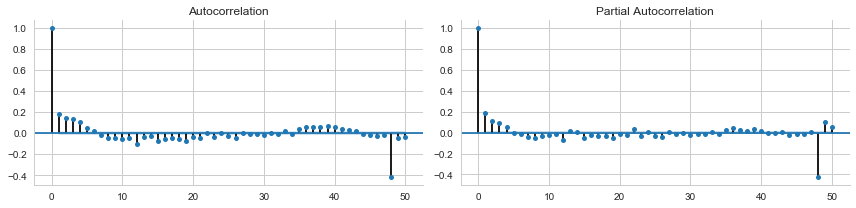
\includegraphics[width=0.95\linewidth]{demand_ACF_diff.png}
   \caption{ACF/PACF plot for demand variable}
   \label{fig:demand_PCF_diff}
\end{minipage}%
\end{figure}

\begin{figure}[H]
\centering
\begin{minipage}{.9\textwidth}
  \centering
  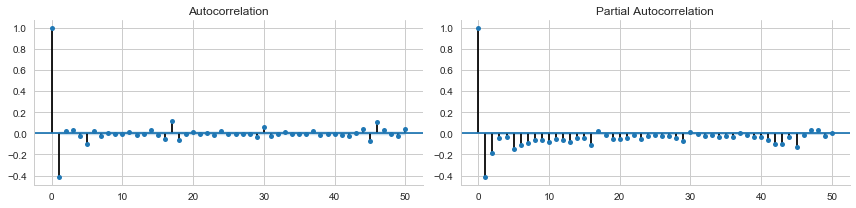
\includegraphics[width=0.95\linewidth]{price_ACF_diff.png}
   \caption{ACF/PACF plot for price variable}
   \label{fig:price_PCF_diff}
\end{minipage}%
\end{figure}

\begin{figure}[H]
\centering
\begin{minipage}{.9\textwidth}
  \centering
  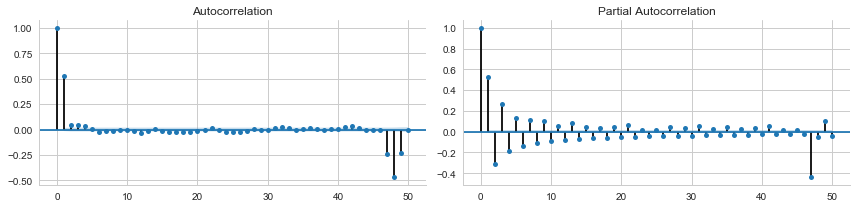
\includegraphics[width=0.95\linewidth]{temp_ACF_diff.png}
   \caption{ACF/PACF plot for temperature variable}
   \label{fig:temp_PCF_diff}
\end{minipage}%
\end{figure}

\noindent In order to test if the data is now stationary we used the Augmented Dickey Fuller (ADF) test. This test has a null that there is a one unit root time series so a rejection of this suggests stationary data. The results rejected the null and provided us with some evidence that we had successfully transformed the data into stationary.

\subsection{Machine Learning EDA}
\label{section:machine_learning_eda}

EDA was also conducted on the lagged demand features and the dummy variables created in this section. As expected, this analysis did not reveal any interesting conclusions due to the similarity in the features. For instance, the variable, `lag\_2' has identical observations to `lag\_1', except that is has been shifted in time by a single period. The only differences in the data were related to the dummy variables. For example, the power demand in Winter was higher than the reference season of Autumn, as expected. Regardless, a small subsample of the plots, are provided in Appendix \textbf{(insert reference)}, for reference.

% Include ADF results in the Appendix

\section{Modelling}
\label{section:modelling}

This section outlines the various modelling techniques used to accurately predict the 30 minute ahead power demand within South Australia. Namely, several classes of models were considered, including: baselines - random walk and industry standard models for comparative purposes, time-series models - traditional forecasting methods, machine learning models - evaluating complex non-linear models such as neural networks, and simpler linear models such as linear regression.

\subsection{Model selection criterion}
\label{section:model_selection_criterion}

We selected two metrics to assess the performance of our models.
The Mean Absolute Percentage Error (MAPE) and the Mean Absolute Error (MAE). According to \citet{kotillova_statistical_2012} these are the two most common metrics for reporting electricity forecasting in industry and academic settings respectively. Using these metrics we aimed to find the best linear model and the best neural network model using the validation set.
\\
\\
On the other hand, the time-series models used either the Akaike Information Criterion (AIC) or visual identification for model selection. For instance, the order selection for ARIMA models could be achieved using ACF and PCF plots as per the previous section, or using an automatic selection process based on AIC. 
\\
\\
Nonetheless, using the test set, the best machine learning model and the best time-series model could be compared against the industry models the the time-series benchmarks. For this particular activity, the MAPE and MAE were reported for the test period outlined in Section \ref{section:data_split} in Table \ref{table:data_split}.

\subsubsection{MAPE}

MAPE is considered the ``preferred metric by [power] industry forecasters" \citep{kotillova_statistical_2012} and will be our primary model selection measure. It is widely used due to its simplicity and ease of comparison between models as it expresses accuracy as a percentage. The scale independence of MAPE is a advantage compared to MAE. The MAPE is defined as per Equation (\ref{eqn:mape}).

\begin{equation}
\label{eqn:mape}
MAPE = \Big(\frac{1}{n} \sum_{j=1}^{n} \frac{|y_j - \hat{y_j} |}{y_j} \Big) \times 100
\end{equation}

\noindent The MAPE does have a few limitations that need to be considered when using it. To prevent division by 0 none of the demand values can be 0, we have protected against this by filling any missing values with reasonable replacements as power demand should never be zero. The other issue is that the measure puts a higher penalty on overestimated values compared to under estimated values. This can lead to a tendency to select models that under forecast values over a model that over forecasts. In our circumstance under estimation of demand is problematic so we consider MAE alongside MAPE.

\subsubsection{MAE}

MAE is a widely used metric by researches in time series analysis that estimates accuracy by averaging the absolute errors of prediction. It is defined as per the following equation,

\begin{equation}
\label{eqn:MAE}
MAE = \frac{1}{n} \sum_{j=1}^{n} |y_j - \bar{y_j} |.
\end{equation}

\noindent MAE is a scale dependent metric meaning that it produces results in the same scale as the data being measured. Therefore, caution should be used when comparing models with transformations applied. 

%if time add more ad and dis on MAE



\subsection{Justification for models selected}

Based on the paper by \citep{kotillova_statistical_2012}, we have tried four baseline models for comparison. These are naive prediction methods. The best performing baseline model was the random walk one step ahead. This makes sense as most time series processes are dependent on prior outcomes.


%Justify WHY RW one step ahead make sence:

%based on the markov Chain(a stochastic model describing a sequence of dependent events),  intuition: most thins in the real world are clearly dependent om prior outcomes,. RW one step ahead is short-term memory for the most recent event only. 

%might also briefely discuss relevant advantage / disadvantage of ML method and statistical method

\subsection{Industry standard model}

Based on the paper by \citet{kotillova_statistical_2012}, we use their definition of the industry model. This model predicted one step ahead t+1 demand using:
\begin{enumerate}
\item The previous 5 lags (t, t--1, t--2, t--3, t--4)
\item The same time (t+1) in the previous week 
\item The previous 5 lags in the previous week
\end{enumerate}

\noindent These features have a logarithmic transformation applied then the differences between the successive values are calculated. This is leads to a model with 9 features (Sharmsollahi et al., 2002).
\\
\\
This industry model is used to predict 5 minute ahead demand for the New England area (located in America). Different data sources are used to train this model so it does have some limitations when comparing against our model. Despite this model being used used in a different context to the Adelaide demand 30 minute ahead prediction modelling we still believe it acts as a good industry benchmark.

\subsection{Time series models}
We considered a wide range of time series models including Seasonal Exponential Smoothing (ES), Seasonal ARIMA, Bayesian structural time series (BSTS) and Auto regressive (AR) models. We discarded ES as it performed very poorly in all measures of accuracy suggesting that ES models are not appropriate for this data. ARIMA and BSTS models could not beat AR model performance and were discarded due to their complexity In ARIMA models our seasonality is 48 periods (one day) which makes the rolling window method very slow and BSTS modelling takes even longer to train without much improvement in performance. Due to these limitations we discard them and focus on the best performing model, AR.

\subsubsection{Auto Regressive models}

AR models use a linear combination of the output variable's previous values to forecast future values. In this case we use the previous values of demand in order to predict the next value of demand. AR models can be expanded to include seasonality. In order to select the number of lags (p) to include in the model we use the partial autocorrelation plot to select the maximum lag as the one beyond where the PACF goes to zero. An AR(p) model is of the form shown in Equation \ref{eqn:AR} where the prediction is based on a weighted value of the previous demand value.

\begin{equation}
\label{eqn:AR}
 X_t = c + \sum_{i=1}^p  \phi_i X_{t-i} + \epsilon_t 
\end{equation}


\noindent AR models can be expanded to include seasonality. Hence when there is seasonality the stationary assumption is violated as the average demand during summer is higher then in winter. In order to address this seasonal differencing is required which removes any trend to produce stationarity.

% AR(1), Ar(48) and AR(336)
% AR(336) is very good! Intuitively, there are two reason:
%% 1, based on complex seasonality plot (figure 3), stronger in-week seasonality, compared to in-day seasonlity
%% 2, also based on the lagged power demand bar plot (figure 14,15 ) lag 336 has strong ,,,,
%% 3, consistent with the MAPE, and AIC results of AR(1), Ar(48) and AR(336) (see notebook)

%\subsubsection{Seasonal exponential smoothing}

%Exponential smoothing methods use weighted averages of past observations using a rolling window. The weights decay exponentially the further in the past the data is. These models are based on the assumption that newer data is more valuable for forecasting then older data. Based on the paper titled \textit{Statistical and Machine Learning Methods for Electricity Demand Prediction} the Holt-Winters' seasonal method was considered. This model is built from a forecast equation, a level smoothing equation, a trend smoothing equation and a seasonal smoothing equation.   

%\subsubsection{Seasonal ARIMA}

%AutoRegressive Integrated Moving Average (ARIMA) models combine autoregressive and moving average models into a single technique. Autoregressive models use a linear combination of predictors to forecast the variable of interest while moving average models uses past forecast errors to create a regression model. ARIMA models can be expanded to include seasonality. A key assumption of to apply ARIMA models is stationary. Hence when there is seasonality this assumption is violated as the average demand during summer is higher then in winter. In order to address this seasonal differencing is required which removes any trend to produce stationarity.

\subsection{Machine Learning Methods}

\subsubsection{Linear regression}
\label{assumptions}

Multiple linear regression (MLR) is basic model useful as a comparison between other models. The key assumptions for the model to be valid as as follows.
\begin{enumerate}
\item Linear: the time series follows a model which is linear in its parameters 
\item Zero conditional mean: expected value for error term is zero if we have all the data.
\item No perfect collinearity: no independant variable is constant or a perfect linear combination of the others.
\item Homoskedasticity: errors have constant variance across time
\item No correlated errors: errors in two different time periods are uncorrelated
\item Independent and identically distributed errors
\end{enumerate}

\noindent These assumptions are rarely satisfied in practice, particularity the linear assumption. It is important to check these assumptions to give context to the MLR model results. Therefore we consider methods such as variable selection and shrinkage methods to improve MLR. 
\\
\\
\textbf{Shrinkage methods: Ridge regression}

\noindent Ridge regression is a shrinkage method that introduces the tuning parameter $\lambda$ into the least squares fitting procedure. This parameter adds a $l_2$ norm penalty term, $\lambda \sum_{j=1}^{p} \beta_j^2$, to the coefficients to drag them towards zero. The purpose of this penalty is to reduce the variance of the prediction with a small increase in bias (James et al., 2015). Ridge regression works best when the least squares estimates have high variance. However the tuning parameter will never decrease a parameter to 0 and therefore cannot perform variable selection. When these variables are not all important Ridge will retain them and produce a less interpretable model. The tuning parameter is chosen using cross validation to select the best value.
\\
\\
\textbf{Shrinkage methods: LASSO}

\noindent The Least Absolute Shrinkage and Selection Operator (LASSO) was developed to address the limitation of Ridge regression that all p predictions are included in the model. LASSO is able to perform variable selection by forcing some coefficients to 0 if the tuning parameter is large enough. To do this it adds an $l_1$ norm penalty term $\lambda \sum_{j=1}^{p} |\beta_j|$ to the residual sum of squares. The result is a model that is easier to interpret with a reduction in variance and slight increase in bias. The tuning parameter is also chosen via cross validation. A disadvantage of this model is that in situations where none of the true parameters are equal to zero LASSO can exclude these variable leading to worse prediction.
\\
\\
\textbf{Shrinkage methods: Elastic net}

\noindent Elastic net attempts to combine the advantages of Ridge and LASSO by including both a $l_1$ and $l_2$ norm penalty term. The result is a shrinkage method that can still perform variable selection like LASSO and reduces coefficients of correlated predictors like Ridge regression. 

\subsubsection{Neural networks}

Neural networks are a machine learning method inspired by the interconnected node structure of human neurons. In their most basic form neurons receive information from input nodes, process the information in some way and produce an output (Hippert et al., 2001). They have the advantage of being incredibly adaptive to complex patterns due to their non-parametric nature. They make no assumptions on the structure of the input data and are usually able to `learn' complex patterns much better than traditional methods. The main disadvantage of neural networks is they act as a black box which makes it hard to interpret the model. 

\subsection{Time series: Model selection and diagnostics}
% Write time-series model assumptions. 
The classical linear model assumptions for time-series regression are what AR and linear models are based on. See section \ref{assumptions} for the assumptions.
% AR model and Linear ridge model all Based on it 



%\subsubsection{BSTS models}

%[COMING SOON]


\subsubsection{Auto regressive models}

Based on the results from our complex seasonality plot in section 4.3, as the weekly seasonality seems stronger than daily seasonality, we try three AR candidates. AR(1), AR(48) (in-day seasonality) and AR(336) (in-week seasonality).
\\
\\
\textbf{AIC}

%% overfitting
%% for AR(336), it is intuitively could be overfitting as more than 300 parameter makes model can be quite complexity, but we can justify the overfitting could be not a issue here as firstly, based on MAPE result, AR(336) peformance well. Secondly, our data is quite high frequency, the simplest in day seasonlity is already 48 , so AR(336) in our case is reasonable. (i.e. much higher lag order than weekly/monthly/yearly data is really reasonable)

\noindent With larger lags AIC always decreases in the training data so that when lag reaches 336 AIC approaches 0, shown in Figure \ref{fig:AR_AIC_train} (appendix). Therefore selecting the model with the lowest AIC will just select the most complex model and may result in overfitting. Hence we also considered AR(48) as we observed a large decrease in the AIC plot at p=48 (Figure \ref{fig:AR_AIC_train}). 
\\
\\
Despite these concerns of overfitting the fact that our data is such high frequency makes AR(336) reasonable despite containing over 300 parameters.

% For AR model, I think table 2 and fogure 9 and 10 (acf plot for residual) is enough, can put other plots in appendix

%% tell yiran , can put figure 9 and 10 in the same line if needed.




\begin{table}[H]
\centering
\caption{AR Models AIC: training data}
\label{table:hyperparameter_optimisation_results}
\begin{tabular}{@{}cccc@{}}
\toprule
 & \textbf{AR(1)} & \textbf{AR(48)} & \textbf{AR(336)} \\ \midrule
AIC & 37689.72 & 164 & 0.003 \\ \bottomrule

\end{tabular}
\end{table}

\noindent \textbf{ACF}

\noindent After these 3 models were chosen for consideration we performed a residual check using an ACF plot. The AR model that satisfies the residual check was AR(336) shown in figure \ref{fig:ACF plot for AR(336)}. All of the remaining ACF plots are available in the appendix (Figures \ref{fig:ACF_plot_AR(1)} and \ref{fig:ACF plot for AR(48)}). 

\begin{figure}[H]
\centering
\begin{minipage}{.5\textwidth}
  \centering
  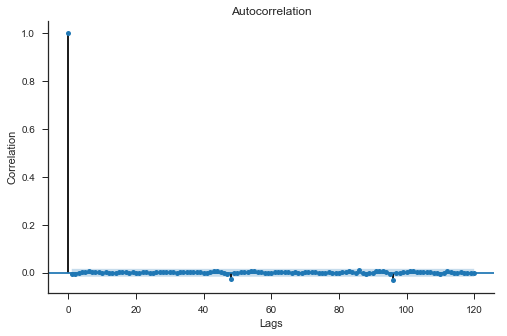
\includegraphics[width=0.95\linewidth]{ACF_AR_336_.png}
   \caption{ACF plot for AR(336)}
   \label{fig:ACF plot for AR(336)}
\end{minipage}%
\begin{minipage}{.5\textwidth}
  \centering
  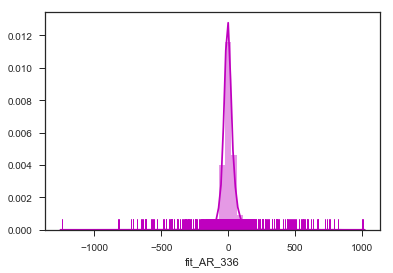
\includegraphics[width=0.95\linewidth]{AR_hist.png}
   \caption{Histogram and kernel density estimate for AR(336)}
   \label{fig:Histagram and kernel density estimate for AR(336)}
\end{minipage}
\end{figure}

%% Based on ACF plot, we can say there is no sereal correlation in residuals. (seems small pattern at 48, 96 etc, but it is really ok enough.)

% \begin{figure}[H]
% \centering
% \begin{minipage}{.75\textwidth}
%   \centering
%   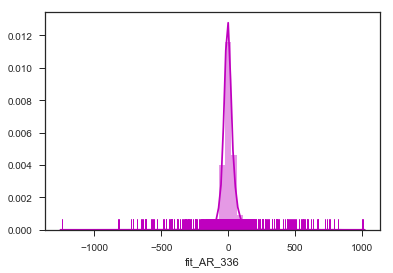
\includegraphics[width=0.95\linewidth]{AR_hist.png}
%    \caption{Histogram and kernel density estimate for AR(336)}
%    \label{fig:Histagram and kernel density estimate for AR(336)}
% \end{minipage}%
% \end{figure}




\noindent Based on these plots we select AR(336) as this model best satisfies the assumptions of stationarity and normal distribution. There is some evidence that there is still some outliers based on the long tail potentially not completely satisfying the white noise assumptions (see Figure \ref{fig:Histagram and kernel density estimate for AR(336)}) .However this model satisfies our assumptions the best. The overfitting might be a problem in the AR(336) model due to too many estimated parameters, but considering that our dataset is high frequency and the simplest in-day seasonality includes 48 observations already, 336 order should be reasonable here. 
\\
\\
Our model selection and diagnostic processes considered a variety of AR models but we focus our further testing on the AR(48) and AR(336). AR(1) has very poor AIC performance and ACF plot so we drop it from consideration.

\subsection{Machine learning: Model selection and diagnostics}

\subsubsection{Linear Models}

The hyperparameters for the linear models were selected using cross-validation (CV) for our three regularised linear models. CV provides an estimate of the out-of-sample MSE. We used 5-fold CV on the training data to select the complexity parameters. 5-fold CV randomly partitions the data into 5 groups using 1 fold as the proxy validation set and the remaining 4 as the training set. The MSE is calculated on the observations in the left out fold and the procedure is repeated for each fold. The final CV MSE is an average of the results for each fold. We used k fold CV as it is less computationally expensive compared to leave one out cross validation. 
\\
\\
The hyperparameters selected for the three regularised linear models are shown in Table \ref{table:hyperparameters_linear}.

\begin{table}[H]
\centering
\caption{Linear Models: Hyperparameter Selection}
\label{table:hyperparameters_linear}
\begin{tabular}{@{}cc@{}}
\toprule
 & \textbf{Hyperparameter/s} \\ \midrule
Ridge & $\alpha=1.400$ \\
LASSO & $\alpha=0.165$ \\
Elastic Net & $\alpha=0.057$, $l_1$ ratio = 1.000 \\ \bottomrule
\end{tabular}
\end{table}

\noindent What is interesting about Table \ref{table:hyperparameters_linear} is the choice of $l_1$ ratio for the elastic net model. By selecting a value of 1, the elastic net model essentially moves towards the LASSO model. Therefore, we expect these two models to have similar results.
\\
\\
These complexity parameters shrink the coefficients for the ridge and elastic net models, and may also have the effect of removing coefficients all together for the LASSO and elastic net cases. Nonetheless, as will be described in the next section, the ridge model has the highest performance on the validation data, therefore only its coefficients are interpreted here. Figure \ref{fig:ridge_co} shows the ridge model coefficients.  


\begin{figure}[htpb!]
\centering
\begin{minipage}{.9\textwidth}
  \centering
  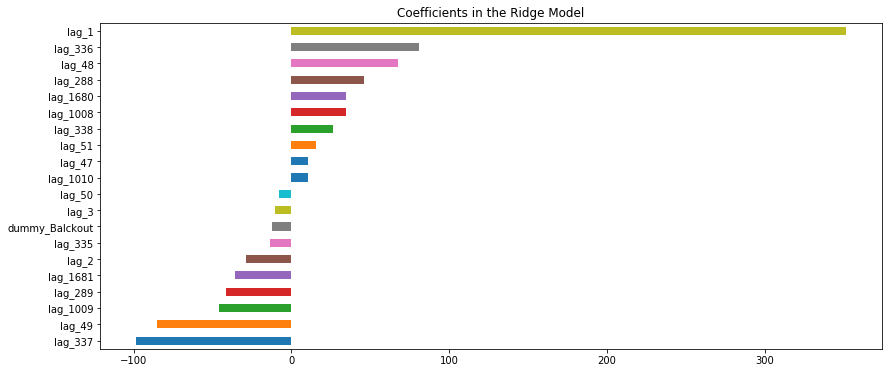
\includegraphics[width=0.95\linewidth]{ridge_co.png}
   \caption{Ridge Regression Coefficient Plot}
   \label{fig:ridge_co}
\end{minipage}%
\end{figure}


\noindent In Figure \ref{fig:ridge_co} larger coefficient, in terms of magnitude, indicates a larger marginal effect on the response. It should also be noted that our model includes both continuous and dummy variables. Where, the continuous variables can take on a larger range of values (not 0 or 1), therefore, they can have a larger impact on the demand prediction. The most important variables selected by ridge were:

\begin{itemize}
\item \textbf{Lag 1}: demand 30 minutes before
\item \textbf{Lag 337}: demand 7 days and 30 minutes before
\item \textbf{Lag 49}: demand 1 day and 30 minutes before
\end{itemize}

\noindent The effect of seasonality when predicting power demand is clear in the ridge regression model. In particular, this model picks up on the weekly and daily seasonality when predicting the 30 minute ahead power. These results are similar to the time-series models, which also used the same seasonality, to make these predictions as well. Despite their differences, it is interesting to note how these types of forecasting approaches have converged to a similar conclusion.

\subsubsection{Neural networks}

Similarly to shrinkage methods neural networks have a range of hyperparameters that need to be selected. These include selecting the number of hidden layers and number of neurons in each layer. These add further complexity to the model and may lead to overfitting. Dropout is used to combat this by randomly removing some neurons from the model. Each neuron needs to have a weight which is applied to the output depending on its importance. These are updated but need to be initialised. Once initialised the weights are updated using an optimiser algorithm. These are updated by running the data through the network a certain number of times known as epochs. Normally the data set is too large to be sent through in a single run so a batch size is also set. All these parameters need to be tunned to minimise the test error.
\\
\\
The hyperparameters were selected using a process of cross-validation randomised grid search. This process follows these steps: 

\begin{enumerate}
\item The hyperparameter space is constructed. This means that all the permutations using the above hyperparameters are found which is a very large set of options 
\item A random number models are selected from this hyperparameter space (75 in this case) 
\item Each model undergoes 3-fold cross validation to find the MSE for each fold on the training data.
\item Take the mean of the 3-folds for each of the 75 models
\item Select the 3 models which have the lowest mean CV score based on the MSE
\end{enumerate}

\noindent The parameters of the 3 best models are outlined in Table \ref{table:hyperparameter_optimisation_results} in Appendix \ref{appendix:nn_validation_models}. These are the three models which will be tested alongside the linear and time-series models on the validation data.


\section{Model Validation}

The goal of this section is to identify the best performing models on the validation data to identify the best: linear model, NN model and time-series model. 

\subsection{Validation results}

\subsubsection{Linear models}

The model validation results for linear models are shown in Table \ref{table:model_validation_linear}.

\begin{table}[H]
\centering
\caption{Model Validation Results for the Linear Models}
\label{table:model_validation_linear}
\begin{tabular}{@{}ccccc@{}}
\toprule
 & \textbf{MLR} & \textbf{Ridge} & \textbf{LASSO} & \textbf{Elastic Net} \\ \midrule
MAPE (\%) & 1.80 & \textbf{1.79} & 28.65 & 28.66 \\
MAE (MW) & \textbf{24.55} & 24.65 & 25.60 & 24.89 \\ \bottomrule
\end{tabular}
\end{table}

\noindent In terms of our primary metric, Ridge models performs the best on the MAPE. Therefore, this will be selected for further model evaluation.
\\
\\
Surprisingly, the MLR model performs well on the validation data (even outperforming Ridge in terms of the MAE). However, this model is expected to have multicollinearity issues as our input variables are the lagged time-series values. Therefore, we don’t expect this model to uphold its assumptions (which Ridge regression overcomes). 
\\
\\
LASSO (and Elastic net which is very similar in this case) both perform really poorly in terms of the MAPE. This is due to the definition of MAPE in Section 5.1 ‘Model Selection Criterion’. Namely, these models are probably mispredicting values which are very close to 0. This “blows up” the MAPE making it get such a large result.
\\
\\
Nonetheless, we select Ridge regression for further evaluation.
\subsubsection{Neural network models}

When training and validating the neural network it became apparent that the choice of dummy variables was inappropriate for this problem. This is in particular reference to the seasonal dummy variables introduced in Section \ref{section:season}. Since this problem required the machine learning models, including the neural networks, to be evaluated against the time-series models, a consistent test was required as introduced in Section \ref{section:data_split}. However, as outlined, this induces sampling bias within the data.
\\
\\
The particular periods which were selected for validation and evaluation were the warmer months. Therefore, power demand was likely to be higher due to increased cooling requirements. However, since the training data did not include many observations where `dummy\_Summer' and `dummy\_Autumn' were equal to 1, the predictions in the out-of-sample set were systematically upwards biased as per Figure \ref{fig:residuals_fitted_nn_withDummy} in Appendix \ref{appendix:nn_residuals}. It is clear from Figure \ref{fig:residuals_fitted_nn_withDummy} that for any given predictions, \textit{all} the residuals are positive, by a significant amount. This is a clear indication that the predictions of power demand are systematically inaccurate by approximately 550MW. This is the effect of not including a dummy variable for the warmer months within the training set. Thus, it is concluded that the use of seasonal dummy variables inappropriate for neural network modeling.
\\
\\
Nonetheless, the validation scores for neural network models, after excluding the seasonal dummies, is shown in Table \ref{table:model_validation_nn}.

\begin{table}[H]
\centering
\caption{Model Validation Results for the Neural Network Models}
\label{table:model_validation_nn}
\begin{tabular}{@{}cccc@{}}
\toprule
 & \textbf{NN 1} & \textbf{NN 2} & \textbf{NN 3} \\ \midrule
MAPE (\%) & \textbf{1.72} & 1.81 & 1.96 \\
MAE (MW) & \textbf{23.65} & 25.60 & 26.32 \\ \bottomrule
\end{tabular}
\end{table}

\noindent NN 1 was our best NN model on the validation data set so we select this model for evaluation on the test data.

% Rewrite the following paragraph after training is complete
%This was a surprising result for the neural network. We expected it to perform better than the linear models due to its higher flexibility however this seems to have over-fit the model to the training data. This explains why the neural network performs less successfully than the time series and linear models. Nonetheless, we select NN model 1.
\subsubsection{Time-series model}

As previously outlined in 6.6.1 the best time series model was selected based on AIC not on validation data as is convention in time series models. This lead us to select AR(48) and AR(336) for further evaluation. 

\section{Model Evaluation}
\label{section:model_evaluation}

Everything in this section is using the test data. Here, we want an idea of how well our model will perform on “unseen” data and how generalisable it is. We also want to compare it to the relevant benchmarks too.

\subsection{Time series models evaluation}
\label{section:performance_metrics}

Table \ref{table:model_validation_time} shows the performance of the time series models on the test data. From these results the best performing model was AR(336). In order to calculate the MAPE and MAE for time series models we used rolling window, with the fixed window length of training data, to calculate the forecast.


\begin{table}[H]
\centering
\caption{Model Evaluation for the time series models by Rolling Window one step ahead}
\label{table:model_validation_time}
\resizebox{\textwidth}{!}{%
\begin{tabular}{@{}cccccc@{}}
\toprule
      & \textbf{AR(48)} & \textbf{AR(336)} & \begin{tabular}[c]{@{}c@{}}\textbf{RW one} \\ \textbf{step ahead}\end{tabular} & \begin{tabular}[c]{@{}c@{}}\textbf{RW Seasonal}\\ \textbf{(In day)}\end{tabular} & \begin{tabular}[c]{@{}l@{}}\textbf{RW Seasonal}\\  \textbf{(In week)}\end{tabular} \\ \midrule
MAPE (\%)  & 2.56   & \textbf{1.83}    & 3.00                                                         & 12.12                                                          & 14.64                                                            \\
MAE (MW)     & 33.58  & \textbf{23.60}   & 39.64                                                        & 161.10                                                         & 194.07       \\   \bottomrule
\end{tabular}%
}
\end{table}

%% AR(1) cannot be better than RW, means that strong serial correlation and bigger lag needed. AR(48) is shows improved forecast accuracy, and AR(336) show really good result, imply that the strong weekly seasonality here! and should be considered in model! 


\subsubsection{Hypothesis Tests for model comparison}

\noindent \textbf{Granger Causality test}
\\
\\
The Granger Causality Test acts as a variable selection hypothesis test. The test checks if adding price or air temperature improves demand forecasting when we are already using demand's history for prediction. From this test we reject the null hypothesis that these variables don't help demand prediction (Appendix Table \ref{table:granger_temp} and Table \ref{table:granger_price}). This suggests that price and temperature have contributed something to the model.
\\
\\

\noindent \textbf{Diebold-Mariano test}
\\
\\
The Diebold-Mariano test compares the forecast accuracy of two forecast methods and acts like model selection.
The null hypothesis is that the two methods have the same forecast accuracy.
\\
\\
From this test we can conclude 
\begin{itemize}
\item AR(336) gives a better forecast accuracy compared to the benchmark model RW one step ahead
\item AR(336) gives a better forecast accuracy compared to AR(48)
\item NN model gives a better forecast accuracy compared to Ridge
\item NN model gives a better forecast accuracy compared to AR(336)
\end{itemize}

These results confirm NN as our best time series model.

\subsubsection{Final model comparison}
\label{final_models}
We selected the best linear, best NN and best time series model. They were compared against the relevant benchmarks and the results are shown in the following table.

\begin{table}[H]
\centering
\caption{Test performance for selected models}
\label{table:model_evaluation_all}
\resizebox{\textwidth}{!}{%
\begin{tabular}{@{}ccccccc@{}}
\toprule
          & \textbf{Ridge} & \textbf{NN Model} & \textbf{Industry}  & \textbf{AR(336)} & \textbf{AR+Ridge} & \textbf{Rand Walk} \\ \midrule
MAPE (\%) & 2.89            & \textbf{1.48}    & 12.60   & 1.83   & 1.61 & 3.00    \\
MAE (MW)  & 38.73         & \textbf{19.72}   & 174.11 & 23.60 & 20.73 & 39.64 \\ \bottomrule
\label{table: test_best3models}
\end{tabular}%
}
\end{table}


\noindent Therefore we conclude that the best model based on both the MAPE and MAE is the NN model. The one step ahead forecast is shown in Figure \ref{fig: NN_plot}.


\begin{figure}[H]
\centering
\begin{minipage}{0.8\textwidth}
  \centering
  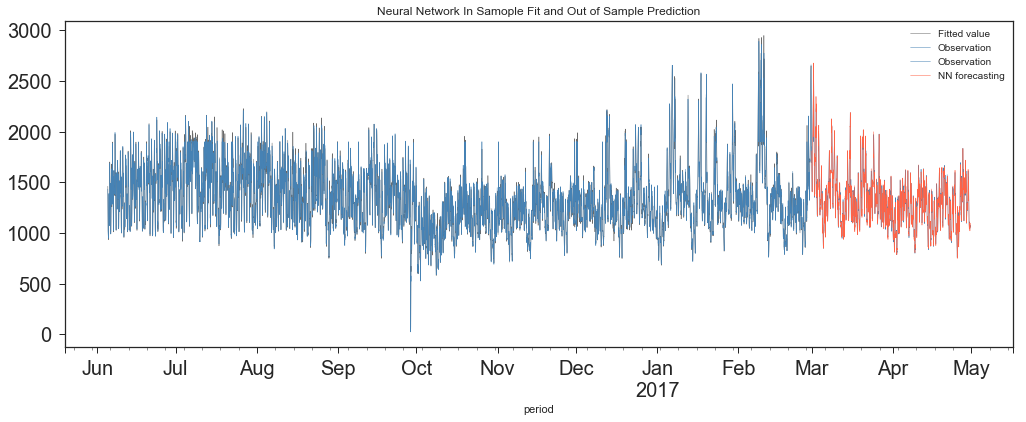
\includegraphics[width=0.95\linewidth]{NN_plot.png}
   \caption{NN one step ahead forecast}
   \label{fig: NN_plot}
\end{minipage}%
\end{figure}


\noindent \textbf{Combination Forecasts Mothod}
\\
\\
\noindent Combining forecasts have been shown in the literature to greatly improve forecasts and also intuitively makes sense as well. If we have two forecasts for the same time period from 2 different models we denote this as  $\hat{y}_{t+1}^{(1)}$ and $\hat{y}_{t+1}^{(2)}$. The respective forecast errors are denoted as $e_{t+1}^{(1)}$ and $e_{t+1}^{(2)}$. From this, letting $\lambda$ be the weight parameter, we denote the combined forecast as:

\begin{equation}
\label{eqn:combined models}
\hat{y}_{t+1}^{c} = (1-\lambda)\hat{y}_{t+1}^{(1)} + \lambda \hat{y}_{t+1}^{(2)}
\end{equation}

\noindent From this, the variance of the combined forecast error is given in Equation \ref{combined_variance}.
\begin{equation}
\label{combined_variance}
Var(e_{t+1}^c) = (1 - \lambda)^2\sigma_1^2 + \lambda^2\sigma_2^2 + 2\lambda(1-\lambda)\rho \sigma_1\sigma_2
\end{equation}


\noindent We can then optimise $\lambda$ to minimise the variance, which gives us Equation \ref{mincombinedvar}
\begin{equation}
\label{mincombinedvar}
\lambda^* = \frac{\sigma_1^2 - \rho \sigma_1 \sigma_2}{\sigma_1^2 + \sigma_2^2 - 2\rho \sigma_1\sigma_2}
\end{equation}


\noindent However, we need to use estimates so we have Equation \ref{combined_variance} where we use $\hat{\sigma}$ as an estimator for $\sigma$,to be the residuals in our estimated model.

\begin{equation}
\label{combined_estimates}
\hat{\lambda^*} = \frac{\hat{\sigma}_1^2 -  \hat{\sigma}_{12}}{\hat{\sigma}_1^2 + \hat{\sigma}_2^2 - 2\hat{\sigma}_{12}}
\end{equation}

\noindent We attempted to combine the best performing models to improve this result further. We considered combinations of our three best performing models; NN with AR, NN with ridge, NN with Ridge and AR. All of these combinations could not improve the MAPE any further than NN alone.  Combining AR(336) and ridge regression did improve the results of either model along which makes our combined AR and Ridge model the second best overall model as shown in Table \ref{table:model_evaluation_all}.

%This provides further evidence that the neural network model has been over-fit to the training data. This instance of the bias variance trade off is demonstrated in this plot which contrasts the drop in MAPE in the training data compared to the validation set over epochs.


%%%%% Rhys will include updated figure here later

% \begin{figure}[H]
% \centering
% \begin{minipage}{.75\textwidth}
%   \centering
%   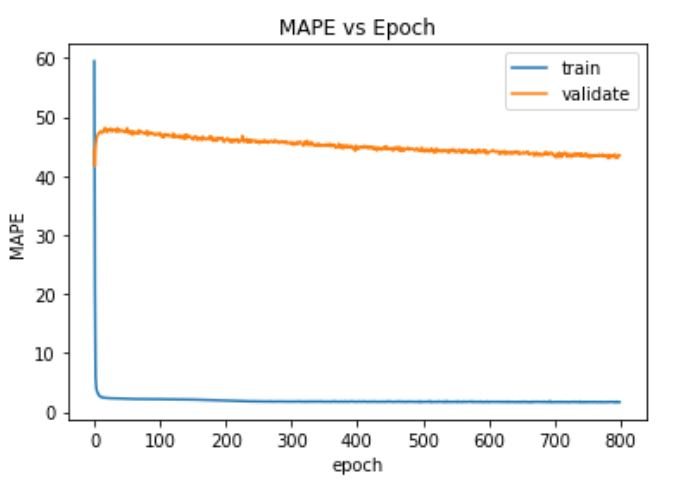
\includegraphics[width=0.95\linewidth]{epoch.JPG}
%    \caption{INSERT CAPTION}
%    \label{fig:ridge_co}
% \end{minipage}%
% \end{figure}



%does the variance in the validation set change compared to the rest of the data

% Furthermore, it could just be the fact that a linear model is better suited to this data. Whereas, neural networks are better at capturing non-linear data. To see if this can be overcome by combining the linear and non-linear effects we added the residuals from the Ridge regression as an input to our NN model. The results are below.

% \begin{table}[h]
% \begin{tabular}{lllll}
%           & NN model with ridge residuals as input &  &  &  \\
% MAPE (\%) & 47.40                                  &  &  &  \\
% MAE (MW)  & 599.04                                 &  &  & 
% \end{tabular}
% \end{table}

% Including the residuals from Ridge regression actually decreased the model performance. This suggests that NN is just inappropriate for this data. Particularly for the period we are trying to test.

%% justify the Time series cross-validation (multiple CV)
%https://otexts.org/fpp2/accuracy.html 

%% FIXED ROLLING WINDOW, ONE STEP AHEAD justification here
%% if Use one-week/one-day ahead, all of them fail
%\begin{table}[H]
%\centering
%\caption{Test Scores for Time-Series Models(Rolling Window one-week ahead)}
%\label{table:time_series_results}
%\begin{tabular}{@{}lllll@{}}
%\toprule
% & \textbf{Bayesian} & \textbf{Seasonal ES} & \textbf{SARIMA} & \textbf{VAR} & \textbf{RW One step } & \textbf{RW One Day} & \textbf{RW One week} \\ \midrule
%MAPE (\%) & 50+ & 100.93 & 50+ & 50+ & 3.004 & 12.116 & 14.635\\
%MAE (MW) & 50++ & 1534.75 & 50++ & 50++ & 39.635 & 161.103 & 194.068 \\ \bottomrule
%\end{tabular}
%\end{table}
\subsection{Statistical inference}

In this section of the report, we are aiming to quantify the uncertainty associated with the results in Section \ref{final_models}. Statistical inference, using a computation resampling method known as bootstrapping, is used to generate a 95\% confidence interval on the test metrics. We perform this on the best performing model, which was the neural network model. Additionally, bootstrapping is used to determine whether the added complexity of the neural network, provides a statistically different result than the simpler ridge model.



\subsubsection{Performance Metrics}


Bootstrapping is used to determine a 95\% confidence interval on the performance metrics (MAPE and MAE). We are going to bootstrap the observations, which is a non-parametric bootstrapping approach, since we are not interested in the model coefficients. In this process, we randomly draw $10,000$ bootstrap samples from the test data and use our best machine learning model to generate predictions. We then compare our predictions to the true power demand values, allowing the MAPE and MAE bootstrap statistics to be calculated. 
\\
% From this, we can calculate the pivotal and percentile 95\% confidence intervals for the Ridge regression as shown in Table \ref{table:ridge_CI}. 

% \begin{table}[H]
% \centering
% \caption{Ridge Regression 95\% CI}
% \label{table:ridge_CI}
% \begin{tabular}{ccc}
% \hline
%  & \textbf{Pivotal} & \textbf{Percentile}  \\ \hline
% MAPE (\%) & (3.00, 3.05) & (2.74, 2.79) \\
% MAE (MW) & (40.35, 41.16) & (36.30, 37.11) \\ \hline
% \end{tabular}
% \end{table}

% The images for this table are in the Drive - ask Rhys where

\noindent From this, we can calculate the pivotal and percentile 95\% confidence intervals for the neural network regression, as shown in Table \ref{table:nn_CI}.

\begin{table}[H]
\centering
\caption{NN 95\% CI}
\label{table:nn_CI}
\begin{tabular}{ccc}
\hline
 & \textbf{Pivotal} & \textbf{Percentile}\\ \hline
MAPE (\%) & (1.53, 1.57) & (1.36, 1.40)\\
MAE (MW) & (19.99, 20.39) & (17.59, 17.98)\\ \hline
\end{tabular}
\end{table}

\noindent If we take the pivotal confidence interval for the MAPE, we can interpret this result by imaging if this investigation was repeated 100 times, then for 95 of those investigations we would find the true population value for the MAPE to be between 1.53\% and 1.57\%. The other intervals can be interpreted in a similar fashion.
\\
\\
Each of the confidence intervals in Table \ref{table:nn_CI} demonstrate variation in the ranges. However, it is a positive sign that each of the four confidence intervals in the table are relatively narrow. The tightness of the intervals is evidence that the neural network produces fairly reliable results, suggesting that it has not been overfit in the training stage. 
\\
\\
Moreover, it is interesting to note that the test statistics calculated for the NN in Table \ref{table: test_best3models} (MAPE=1.48\% and MAE=19.72MW), are not contained in any of the confidence intervals. While unusual, this is not an issue, because using our analogy of the repeated trials from before, this investigation may be one of 5 investigations (out of 100), which do not contain the true population value.
\\
\\
Finally, the high performance of the neural network model is also highlighted in Table \ref{table:nn_CI}. Even with confidence bands applied to the test scores, the upper interval for both the MAPE and MAE are still substantially less than the second highest performing model which was the combined AR Ridge model. Clearly, the ability of the NN to capture the non-linear relationships within the demand data is contributing to the success of its result.
\\
\\
Appendix \ref{appendix:bootstrap} contains the distributions for the bootstrapped MAPE and MAE for the neural network model is shown in Figures \ref{fig:nn_mape_boot_dist} and \ref{fig:nn_mae_boot_dist}.

\subsubsection{Comparison Between Ridge and NN}

We can also extend this bootstrapping process in the previous section to provide a comparison between the ridge regression model and the neural network model. While it would be beneficial to compare the best neural network developed in the study with the industry prediction model, it is clear that the industry model developed is simply inappropriate for 30 minute ahead prediction. Therefore, this section aims to determine whether the added complexity of a neural network model, provides a sufficient enough improvement in terms of predictive accuracy over the simpler ridge model (which would be less prone to overfitting). This time, our bootstrapped statistic is defined as:

\begin{align*}
MAPE_{difference} = MAPE_{ridge} - MAPE_{nn}
\end{align*}

\noindent Since we are trying to minimise the MAPE, we want the statistic to be as positive as possible. Again, we can construct a pivotal and percentile 95\% confidence interval shown in Table \ref{table:CI_ridge_nn}.

\begin{table}[H]
\centering
\caption{95\% CI Comparison Between Ridge and NN}
\label{table:CI_ridge_nn}
\begin{tabular}{ccc}
\hline
 & \textbf{Pivotal} & \textbf{Percentile}\\ \hline
$MAPE_{difference}$ & (1.52, 1.57) & (1.29, 1.34) \\ \hline
\end{tabular}
\end{table}

\noindent Using these intervals, it is also possible to construct a hypothesis test. Where we define our hypotheses as follows:


\begin{align*}
H_0: MAPE_{ridge} &\leq  MAPE_{model}  \\
H_1: MAPE_{ridge} &> MAPE_{nn} 
\end{align*}
\\
\noindent Based on the results in Table \ref{table:CI_ridge_nn}, we observe that the 95\% confidence intervals are both positive (and do not contain 0). Hence, we reject the null-hypothesis at the 5\% significance level, and conclude that we have enough evidence to suggest that the neural network model proposed is statistically significant (i.e. lower MAPE) than the ridge model. This is clear validation that the non-linearity in the South Australian power demand is better modelled using the neural network, and the added complexity is an appropriate trade-off.
%\noindent Since neither of our 95\% confidence intervals for the Ridge case are greater than or equal to the value of 0 we reject the null hypothesis. Therefore, we conclude that the ridge model is an improvement over the industry model in terms of the MAPE.
\\
%However, since both our CI for the NN case are less than or equal to 0, we do not have sufficient evidence to reject the null hypothesis. Therefore, we cannot conclusively say that the NN is an improvement over the benchmark”.

\noindent The bootstrap distribution of this statistic is contained within Figure \ref{fig:diff_mape_boot_dist} in Appendix \ref{appendix:difference_bootstrap}. A similar distribution of the difference has been created for the MAE in Figure \ref{fig:diff_mae_boot_dist}. The resulting confidence interval has a similar conclusion. 

\subsection{Diagnostics}


% \subsubsection{Ridge Regression}

% [REWRITE SECTION]
% \\
% \\
% The ridge regression shows a handful of outliers but generally satisfies the residual assumptions.  
% %Update when Rhys looks at this plot

% \begin{figure}[H]
% \centering
% \begin{minipage}{.5\textwidth}
%   \centering
%   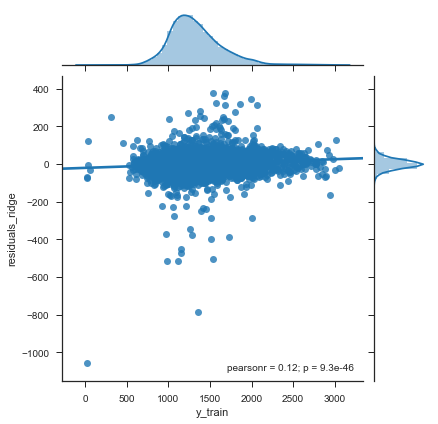
\includegraphics[width=0.95\linewidth]{ridge_residual.png}
%    \caption{Residuals vs. Fitted - Ridge Regression}
%    \label{fig:residuals_fitted_ridge}
% \end{minipage}%
% \end{figure}

%% figure 15 and 16 can combine together, if needed, tell yiran

%\subsubsection{Neural Network}

Neural network models are not constrained by the entire list often prohibitive assumptions imposed on Generalised Linear Models. However, it is still important to complete residual diagnostics to understand deficiencies which may be hold back the predictive accuracy. For instance, Figure \ref{fig:residuals_fitted_nn} shows the residuals vs. fitted values, using the training data. The horizontal axis, at the top of the plot, shows the distribution of the power demand values, whereas the vertical axis plot shows the distribution of the residuals.

\begin{figure}[H]
\centering
\begin{minipage}{.5\textwidth}
  \centering
  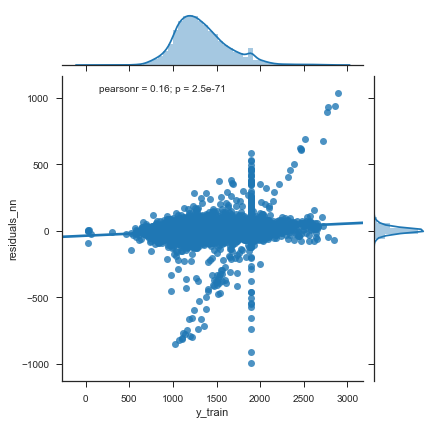
\includegraphics[width=0.95\linewidth]{nn_residual.png}
   \caption{Residuals vs. Fitted - Neural Network}
   \label{fig:residuals_fitted_nn}
\end{minipage}%
\end{figure}

\noindent It is clear from Figure \ref{fig:residuals_fitted_nn} that there are issues with the specification of the model, particularly with the two lines of residuals (vertical and diagonal). These systematic patterns suggest that there are linear relationships in the training data which have not been captured by the neural network. A similar plot is shown for the ridge regression case, in Figure \ref{fig:residuals_fitted_ridge_appendix}, in Appendix \ref{appendix:diagnostics}. From this plot, no clear systematic patterns are observed, suggesting that the ridge model is correctly capturing these linear effects. Hence, the neural network could be improved in the future by combining the predictions with the ridge model to ensure that these linear effects are correctly modelled. These systematic deviations aside, the neural network demonstrates a fairly small range of residuals, with no clear outliers.


%further explaination to be added
%We can also find the outliers for the different models. For instance, the largest 5 outliers for the Ridge model are:

%\begin{table}[H]
%\begin{tabular}{lll}
%DateTime            & Residual (MW) - absolute value & Possible reason                                                                                                       \\
%2017-03-03 15:30:00 & 163.96                         & \begin{tabular}[c]{@{}l@{}}Price change was 400\%\\ Demand change was 4.9\% (\textgreater 75\% quartile)\end{tabular} \\
%2017-03-27 12:00:00 & 116.82                         & Demand change was 4.9\% (\textgreater 75\% quartile)                                                                  \\
%2017-03-27 12:30:00 & 112.35                         & Demand change was 7.1\% (\textgreater 75\% quartile)                                                                  \\
%2017-03-25 13:30:00 & 107.68                         & Demand change was 8.6\%                                                                                               \\
%2017-03-29 13:00:00 & 101.87                         & \begin{tabular}[c]{@{}l@{}}Price was \$0.02\\ Demand change was 10.1\%\end{tabular}                                  
%\end{tabular}
%\end{table}

%The largest 5 outliers for the Ridge model are:


%[INSERT TABLE HERE]

%Clearly, both models are sensitive to sudden changes in the demand (i.e. demand spikes) and price - with the NN being way more sensitive to this. We can plot the distribution of the demand spikes here which seem to be the main influence.

%Sudden changes in demand create sudden changes in price. Therefore, these are basically the same concept.

%[INSERT GRAPH HERE]

\section{Deployment}

\subsection{Trade off between ML model and Time-series model}

Machine learning methods such as NN have the best accuracy. It could be implemented by updating the NN each month or quarter which is avoids having to continually retrain models. This is convienent as retraining the NN model takes significant time and computational costs. However NN models are act as a black box making them hard to interpret due to the complex concepts behind them. This makes them susceptible to overfitting to training data if not implemented successfully. They also require significant feature engineering into to function at the peak potential. This contrasts with Ridge Regression which is easy to understand and interpret however it produces less accurate forecasts.
\\
\\
Time series models also have their strengths in their easy interpretation and low computational cost. The AR(336) model took less than 15 minutes to produce 2 months of predictions. They also are less susceptible to the overfitting problem that machine learning methods have. However they are not as practical for implementation as machine learning methods as they would require frequent updating every half hour.
\\
\\
%In general, machine learning models are forecasting in a "pseudo- cross sectional environment", which contrasts time-series models which work in a 'time series environment'. This 

%we already see lots of benefit of NN model here. roughly speaking, design/learn NN model once can use at least two month, and in practice, might can update model quarterly, which is very convenient and valuable. Learn NN model slowly, but really low computational cost as it can be used in a relatively long period.


% (yiran roughly write)we should also Justify the Computational cost VS accuracy VS Interpretation :

%% ML model: 
%%%% ADV: 
%%%% 1, Best accuracy, 
%%%% 2, and update model can weekly/monthly/quarterly , not need frequently, so very convenient to be used in business. 

%%%% DISadvantage:
%%%% 1, high computational cost each time learn model, 
%%%% 2, hard to interpret and complex concept behind
%%%% 3, a well-designed method, enough feature engineering is necessary, otherwise, overfitting or bad model performance can occur

%% Ridge model: 
%%%% easy to Be understand and interpretation, but less accuracy, and need some feature engineering 

%% Time series models:
%%%% ADV:
%%%% 1. Easy to learn (lean AR(336) model less than 1 secs each time), go though two month test data need only around 15 mins.
%%%% 2. Simple feature engineering needed: only clean data is ok, donot need Build new features(no dummy or lag variales) 
%%%% 3. less risky for overfitting prolem (which is likely to happen in ML model) 
%%%% 4. Easy to Be understand By others 
%%%% 5. easy to interpretation
%%%% DISadvantage:
%%%% 1. lower accuracy, even worse than ridge model, only Beat RW, 
%%%% 2. need update frequently, every half hours, which is not quite reality in real Business case? 


% (detailed reasons)https://towardsdatascience.com/3-facts-about-time-series-forecasting-that-surprise-experienced-machine-learning-practitioners-69c18ee89387

%We select the Ridge Regression model as it performs better than all other models except for the neural network model as measured by MAPE. However as the NN doesn't pass the residual check we conclude the Ridge Regression is a more robust model.

\noindent Hence in order to maximise the accuracy of our forecasts we select neural networks despite their drawbacks in interpretation. 

\section{Literature Discussion}
\label{section:literature_discussion}

It became clear that the results from similar studies were overstated, in particular with the predictive accuracy of neural networks for power demand. For example, the work conducted by \citet{kotillova_statistical_2012} and \citet{bunn_forecasting_2000} both concluded and praised the performance gains which could be obtained by using this type of algorithm. However, these studies failed to correctly partition their data as to prevent overfitting of this algorithm. In both investigations, the data was split into two: training and test data. While this is not uncommon, the paper's alluded to the fact that the test data was used for \textit{both} hyperparameter optimisation and model evaluation. Because of this, their results are likely overfit to the test data, and if their models were to be tested on another out-of-sample set, then they would likely exhibit poor generalisability due to overfitting. 
\\
\\
Moreover, it has been mentioned throughout this report, that modelling the effects of the seasons has been a large challenge to the group. For instance, Section \ref{section:model_evaluation} highlights that the use of seasonal dummies failed to improve predictive accuracy for the machine learning models, due to the way in which the data was partitioned. However, several authors overcame this problem by only analysing the the power demand within a single season (3-month period). For instance, \citet{kotillova_statistical_2012} only looked at the data from Winter, 2010. This meant that the authors did not have to model the complexities associated with the changing seasons, which in turn affects the power demand. Thus, is a major limitation of their work, creating overly optimistic results.


\section{Conclusion}

%\subsection{Research outcomes}

\subsection{Future work}

\textbf{Panel data}: The demand forecast for South Australia could be improved by considering the demand and price of other states. This technique involves combining time series data with cross sectional data to produce a more powerful multidimensional approach to forecasting.
\\

\noindent \textbf{Interval forecasting}: Instead of forecasting a point estimate and the accuracy of that point estimate with measures such as MAPE and MAE future work could consider forecasting Bootstrap intervals. This could provide another dimension of information to energy operators. Also, the bootstrap interval forecasting could be implemented within a rolling window method.

\subsection{Project outcome}

Our best neural network model was able to improve on the industry model by 11.12\%. This equates to savings of about \$25 million for a 10-gigawatt generator \citep{hobbs_analysis_1999}. Improvements of this scale have the potential to have a real life impact for business's and people in Australia. These kind of savings will assist operators to reduce their costs and consumers could benefit with lower power bills in the competitive power market. 

\newpage
\bibliographystyle{agsm} 
\renewcommand{\bibname}{References}
\bibliography{qbus3830_references}
\addcontentsline{toc}{section}{References}

\newpage
%\section{References}
 %need to intent the first reference - Rhys to convert these over time
%\par


%Harvy, B., \& Shepherd, T. (2017). Rolling blackouts ordered as Adelaide swelters in heatwave. News.Com.Au. Retrieved from https://www.news.com.au/national/south-australia/rolling-blackouts-ordered-as-adelaide-swelters-in-heatwave/news-story/18db2b7f2faa9e0308d2a6a0da2d88cc

%How the energy market operates | Energy EXchange. (2018). Retrieved from https://www.eex.gov.au/large-energy-users/energy-management/energy-procurement/energy-pricing/how-the-energy-market-operates


%Potter, B., Macdonald-Smith, A., \& Ludlow, M. (2017). The energy crisis explained: a tragedy in five acts. The Australian Financial Review.Retrieved from https://www.afr.com/business/energy/the-energy-crisis-explained-a-tragedy-in-five-acts-20171004-gytz0s

%Rainfall, temperature and wind forecast and observations. (2017). Retrieved from https://data.gov.au/dataset/rainfall-and-temperature-forecast-and-observations-verification-2017-05-to-2018-04

%Swoboda, K. Energy prices—the story behind rising costs – Parliament of Australia. Retrieved from https://www.aph.gov.au/About\_Parliament/Parliamentary\_Departments/Parliamentary\_Library/pubs/BriefingBook44p/EnergyPrices


%Nau, R. (2014). \textit{Introduction to ARIMA models.}

% Start the appendix section
\newpage
\appendix

\section{EDA}
\label{appendix:further_eda}

\subsection{Time-Series Decomposition}

Figure \ref{fig:demand_before} shows how the time-series for the power demand can be separated into the four components.
\begin{figure}[H]
\centering
\begin{minipage}{.75\textwidth}
  \centering
  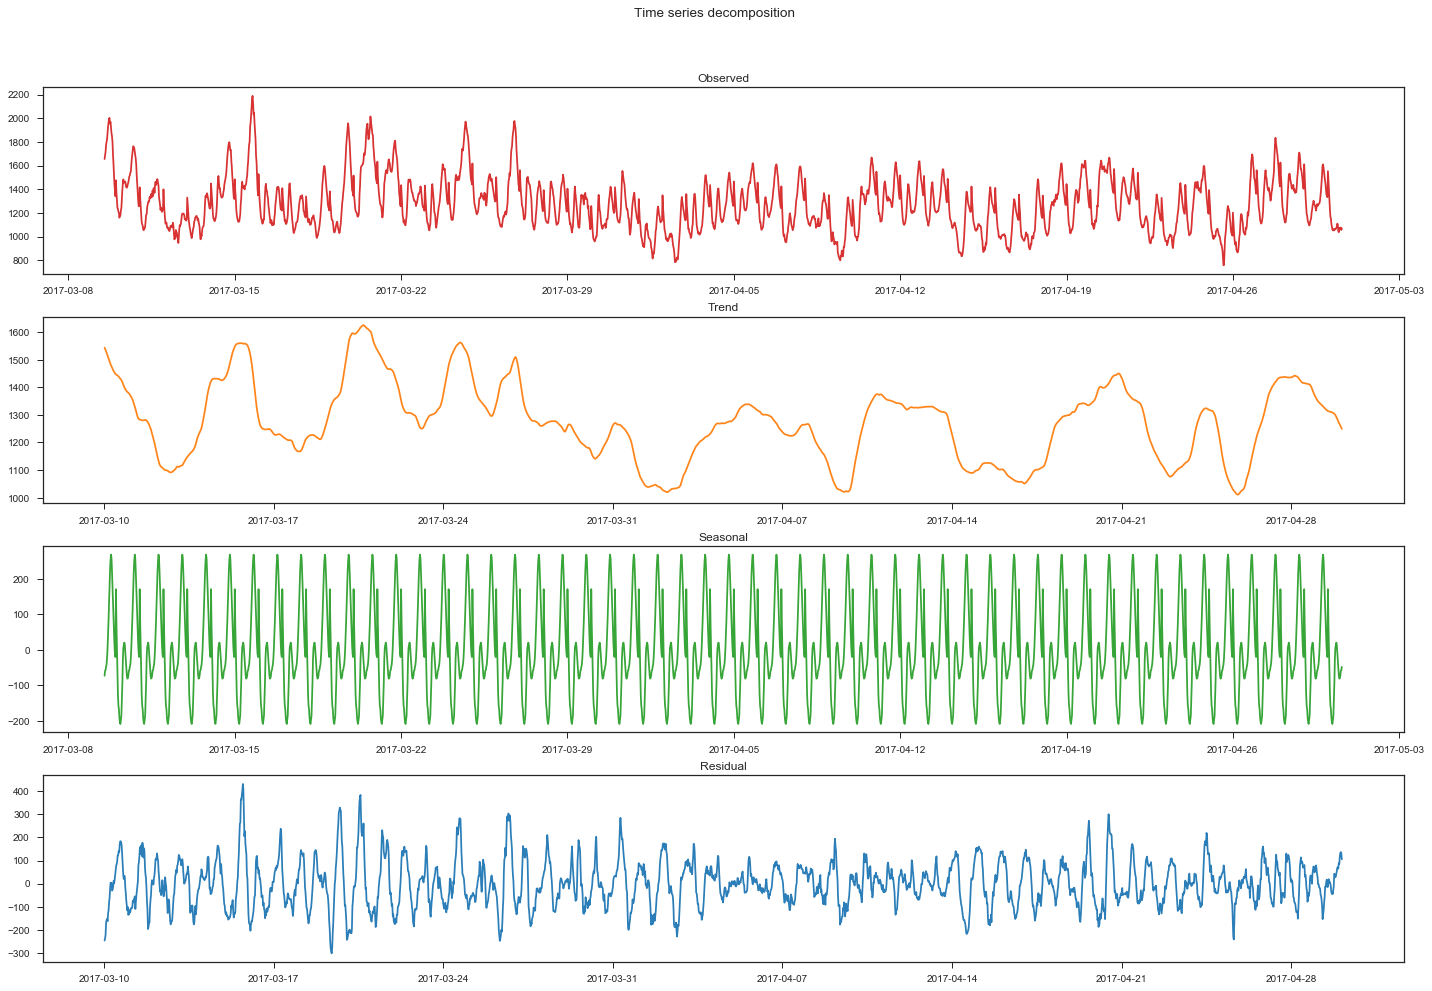
\includegraphics[width=0.95\linewidth]{demand_before.png}
   \caption{Time series decomposition: Demand before outliers removed}
   \label{fig:demand_before}
\end{minipage}%
\end{figure}

\begin{figure}[H]
\centering
\begin{minipage}{.75\textwidth}
  \centering
  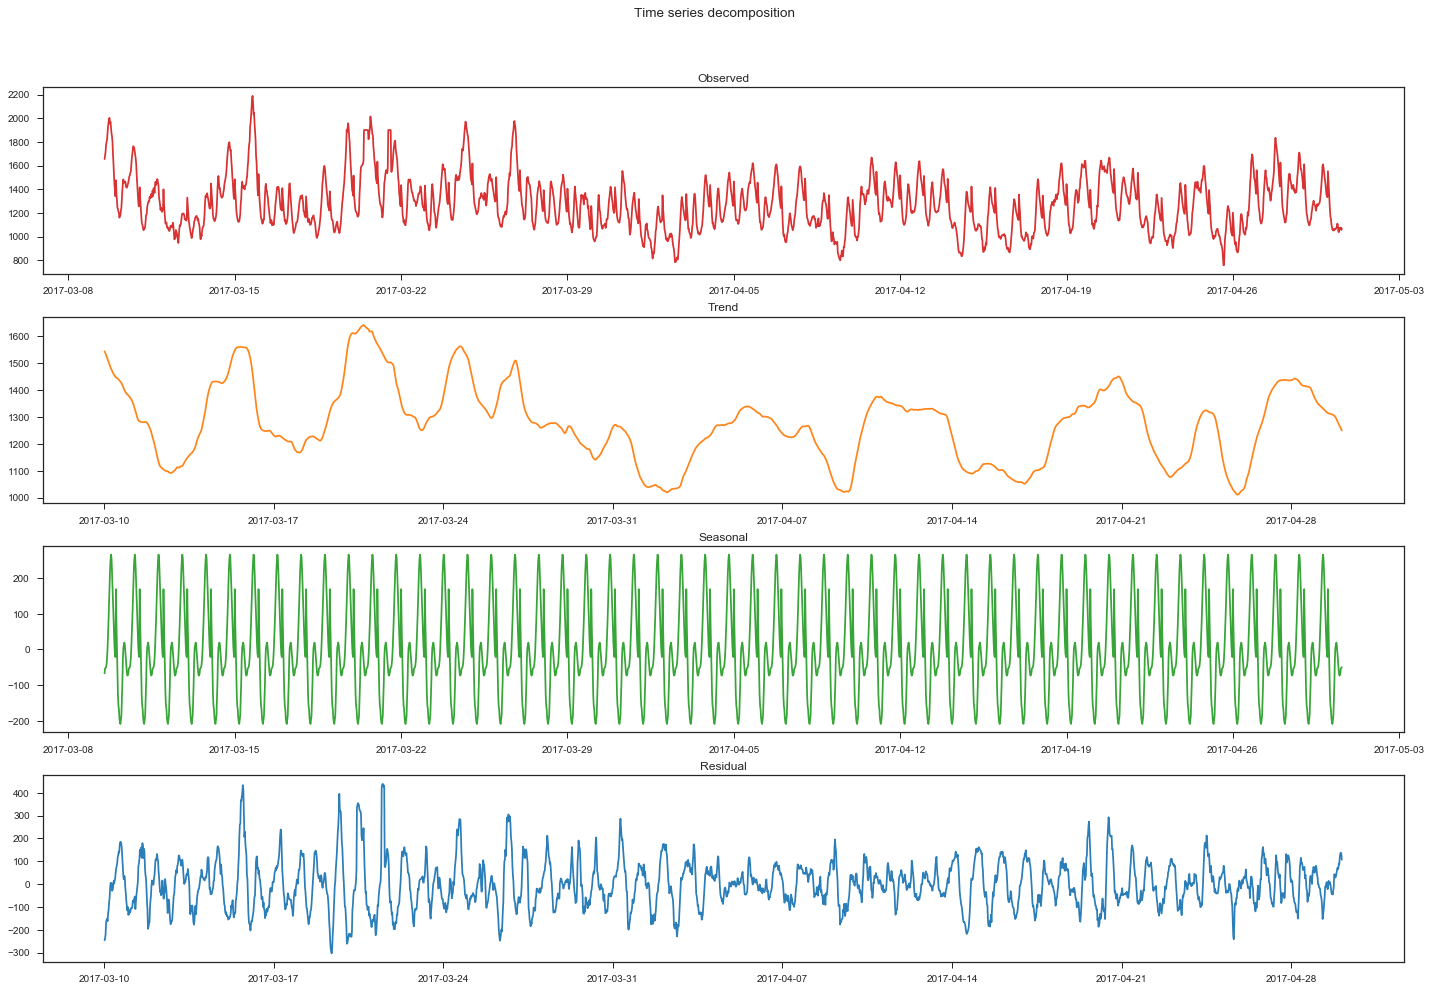
\includegraphics[width=0.95\linewidth]{demand_after.png}
   \caption{Time series decomposition: Demand after outliers removed}
   \label{fig:demand_after}
\end{minipage}%
\end{figure}

\begin{figure}[H]
\centering
\begin{minipage}{.75\textwidth}
  \centering
  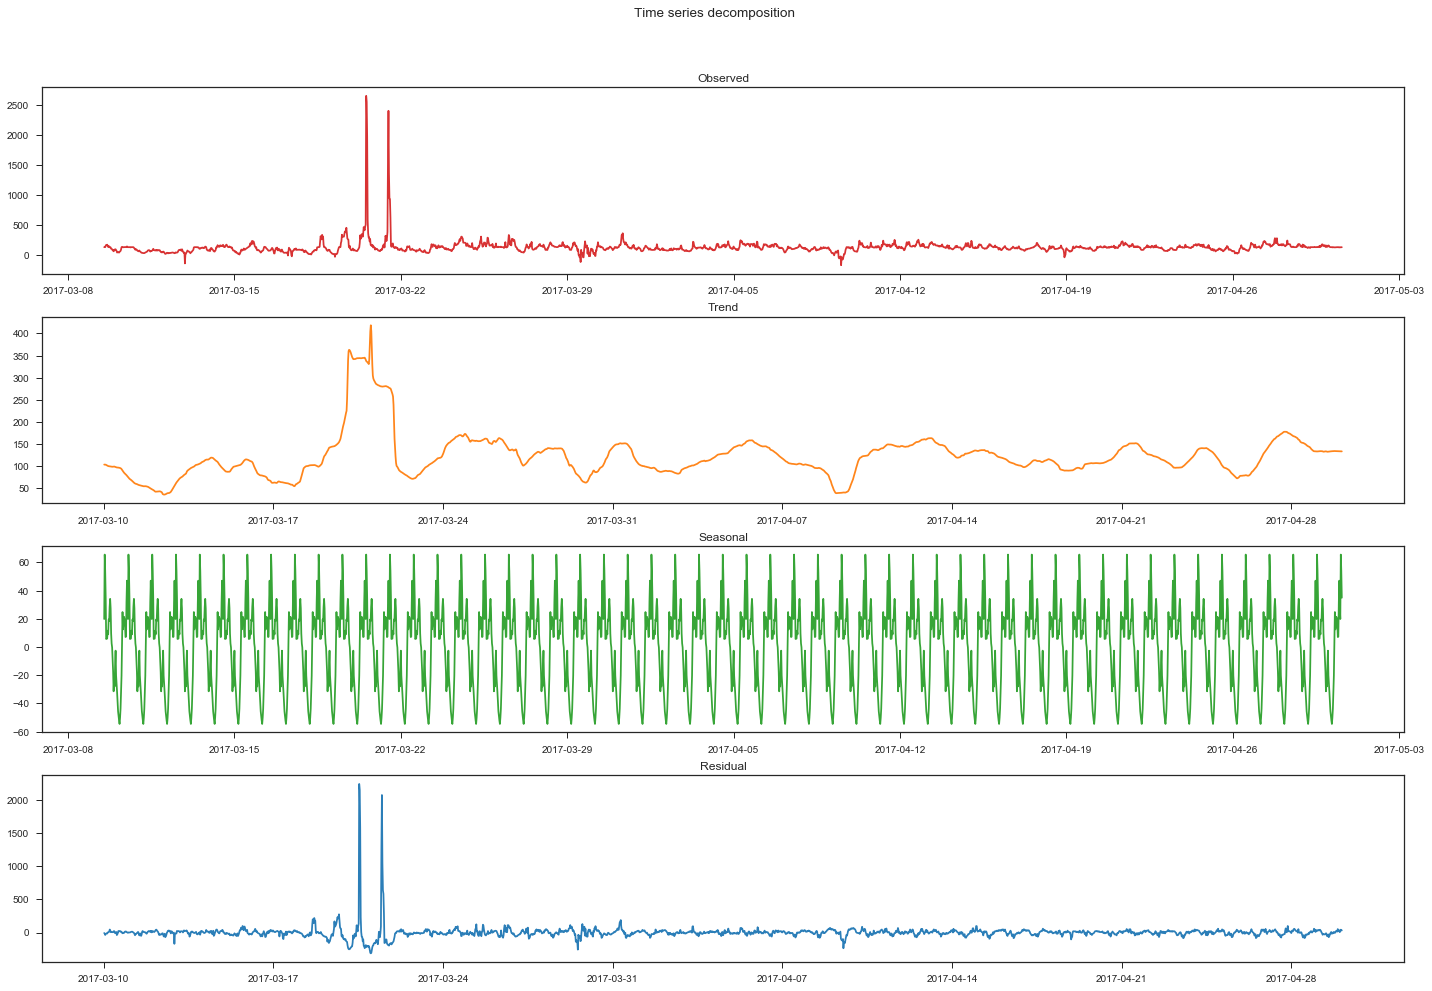
\includegraphics[width=0.95\linewidth]{price_before.png}
   \caption{Time series decomposition: Price before outliers removed}
   \label{fig:price_before}
\end{minipage}%
\end{figure}

\begin{figure}[H]
\centering
\begin{minipage}{.75\textwidth}
  \centering
  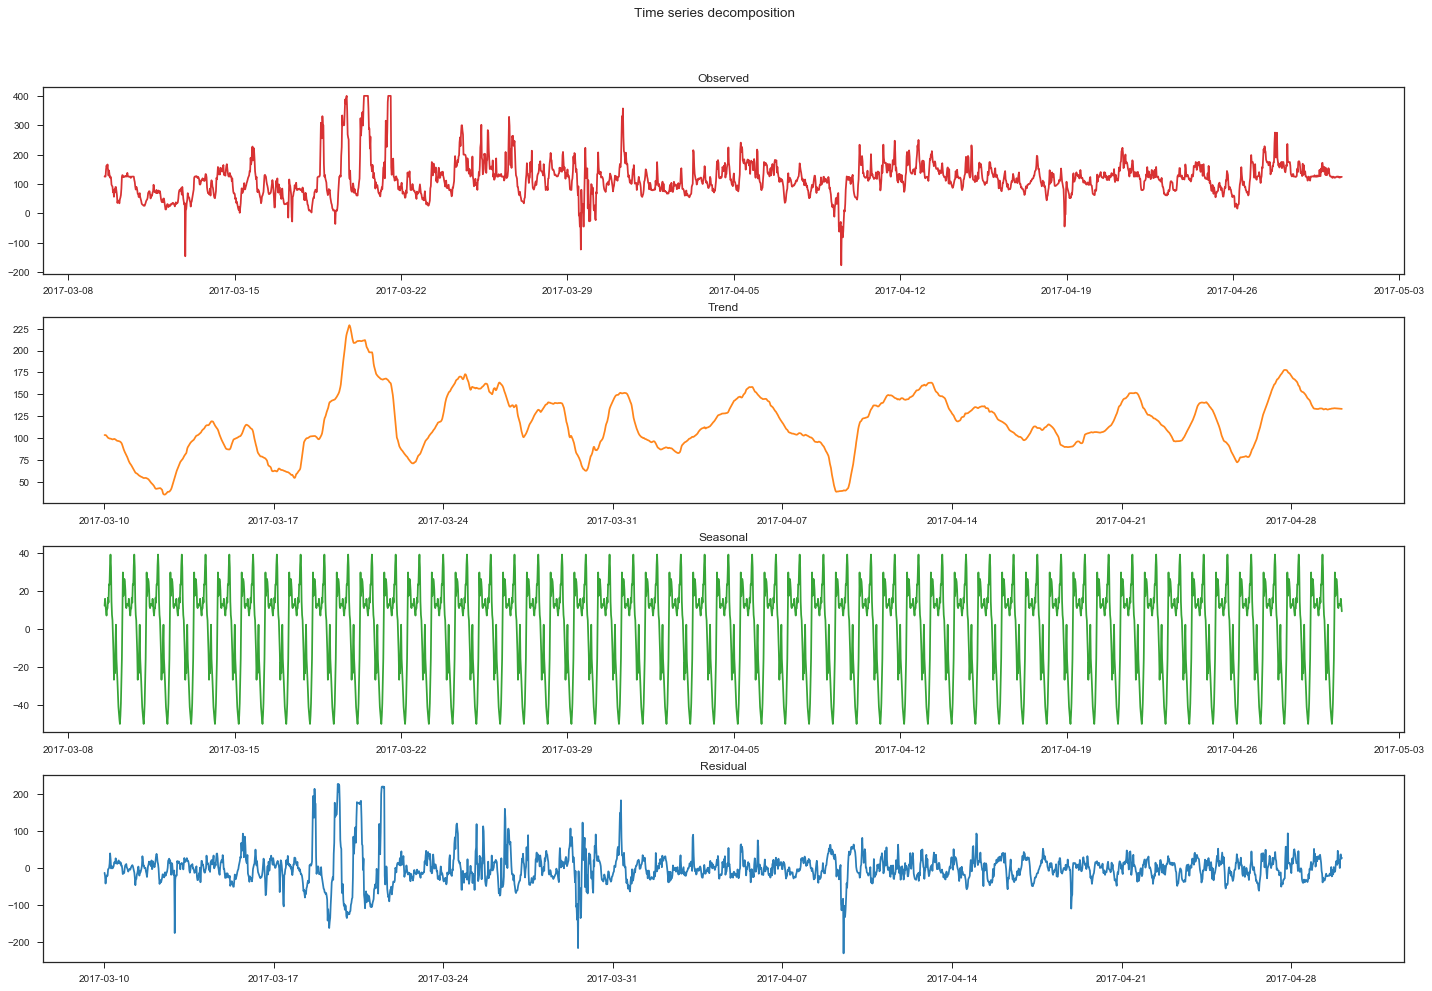
\includegraphics[width=0.95\linewidth]{price_after.png}
   \caption{Time series decomposition: Price after outliers removed}
   \label{fig:price_after}
\end{minipage}%
\end{figure}



\subsection{Machine Learning EDA}
\label{appendix:machine_learning_eda}

When creating the lagged features in the machine learning model, an ACF plot was used to inform which lags were the most correlated with the demand. This is shown in the figure below:

\begin{figure}[H]
\centering
\begin{minipage}{.5\textwidth}
  \centering
  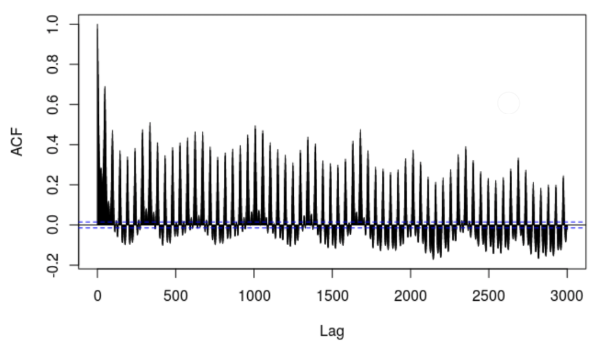
\includegraphics[width=0.95\linewidth]{acf_demand.PNG}
   \caption{ACF Plot of South Australian Power Demand}
   \label{fig:acf_demand}
\end{minipage}%
\end{figure}

\noindent After engineering the features, the following figures show the EDA conducted on the machine learning features. As many of the features contain the same values, they are excluded for brevity.

\begin{figure}[H]
\centering
\begin{minipage}{.5\textwidth}
  \centering
  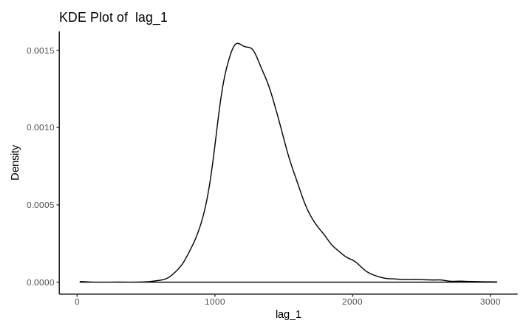
\includegraphics[width=1\linewidth]{lag_1_kde}
   \caption{KDE of `lag\_1'}
   \label{fig:lag_1_kde}
\end{minipage}%
\begin{minipage}{.5\textwidth}
  \centering
  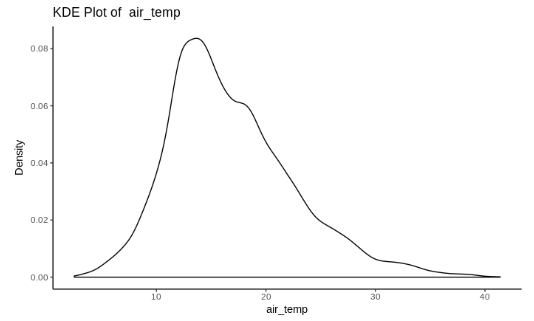
\includegraphics[width=1\linewidth]{air_temp_kde}
   \caption{KDE of `air\_temp'}
   \label{fig:air_temp_kde}
\end{minipage}%
\end{figure}

\begin{figure}[H]
\centering
\begin{minipage}{.5\textwidth}
  \centering
  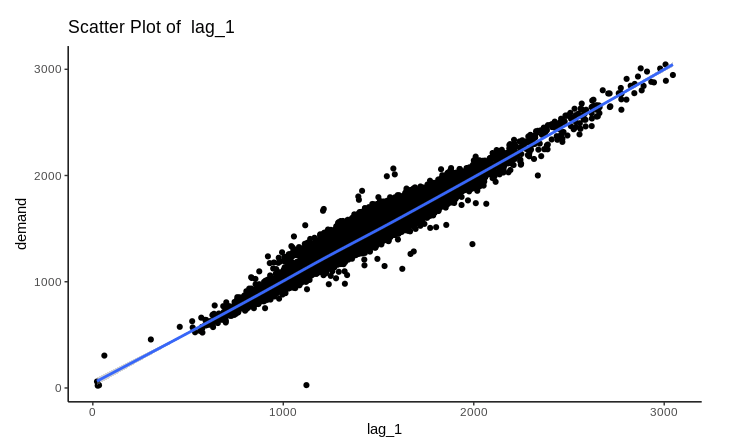
\includegraphics[width=1\linewidth]{lag_1_scatter}
   \caption{Scatter of `lag\_1'}
   \label{fig:lag_1_scatter}
\end{minipage}%
\begin{minipage}{.5\textwidth}
  \centering
  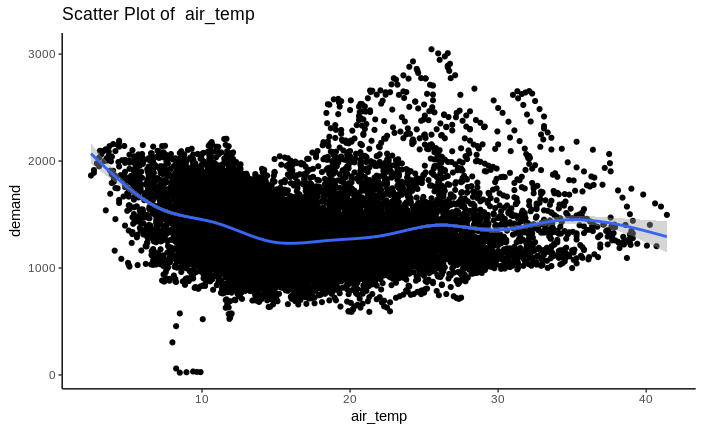
\includegraphics[width=1\linewidth]{air_temp_scatter}
   \caption{Scatter of `air\_temp'}
   \label{fig:air_temp_scatter}
\end{minipage}%
\end{figure}

\begin{figure}[H]
\centering
\begin{minipage}{.5\textwidth}
  \centering
  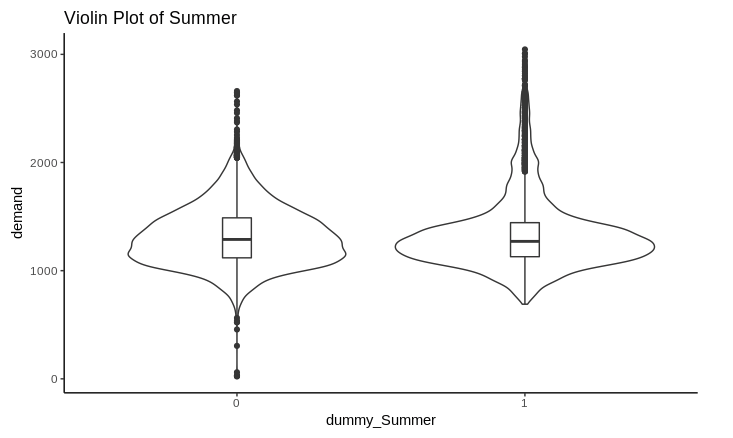
\includegraphics[width=1\linewidth]{summer_violin}
   \caption{Violin of `dummy\_Summer'}
   \label{fig:summer_violin}
\end{minipage}%
\begin{minipage}{.5\textwidth}
  \centering
  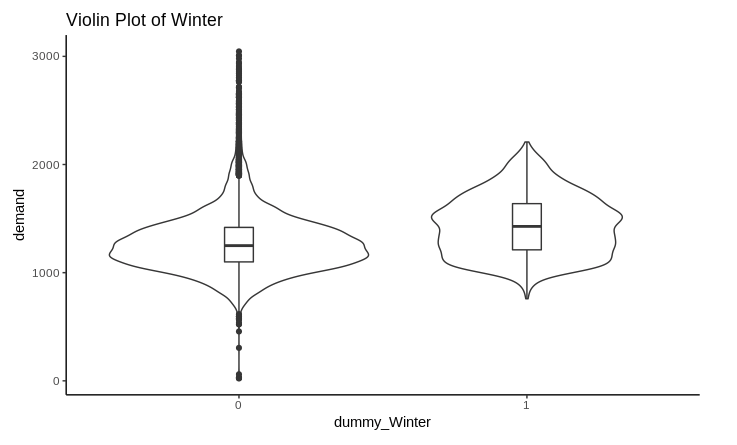
\includegraphics[width=1\linewidth]{winter_violin}
   \caption{Violin of `dummy\_Winter'}
   \label{fig:winter_violin}
\end{minipage}%
\end{figure}

\begin{figure}[H]
\centering
\begin{minipage}{.5\textwidth}
  \centering
  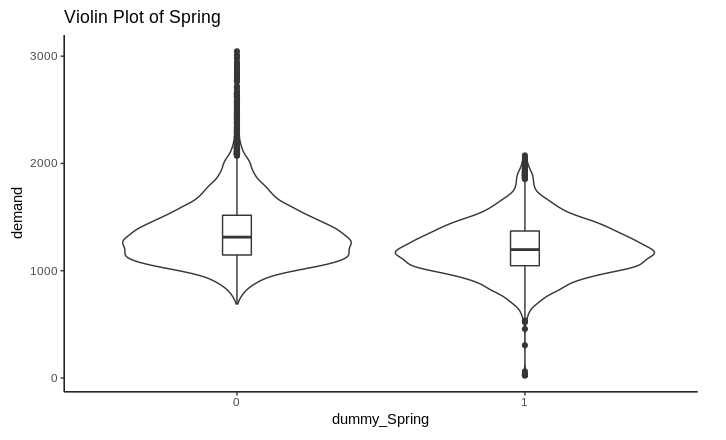
\includegraphics[width=1\linewidth]{spring_violin}
   \caption{Violin of `dummy\_Spring'}
   \label{fig:spring_violin}
\end{minipage}%
\end{figure}

\begin{figure}[H]
\centering
\begin{minipage}{.5\textwidth}
  \centering
  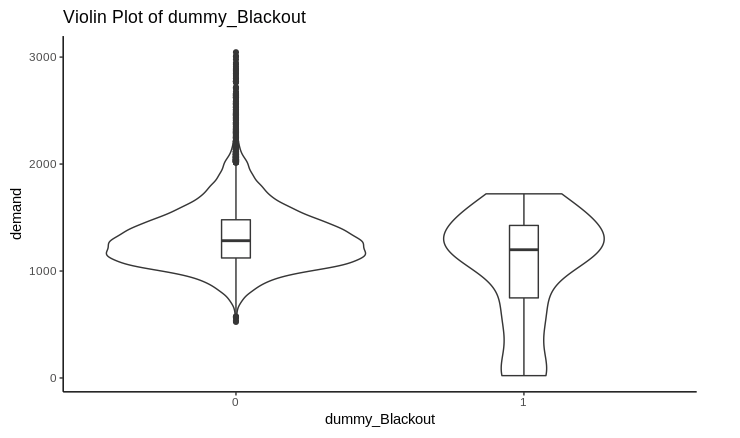
\includegraphics[width=1\linewidth]{blackout_violin}
   \caption{Violin of `dummy\_Blackout'}
   \label{fig:blackout_violin}
\end{minipage}%
\begin{minipage}{.5\textwidth}
  \centering
  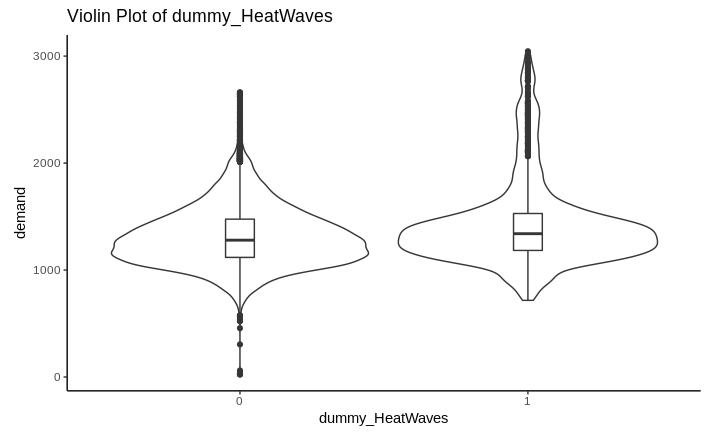
\includegraphics[width=1\linewidth]{heatwave_violin}
   \caption{Violin of `dummy\_Heatwave'}
   \label{fig:heatwave_violin}
\end{minipage}%
\end{figure}

\begin{figure}[H]
\centering
\begin{minipage}{.8\textwidth}
  \centering
  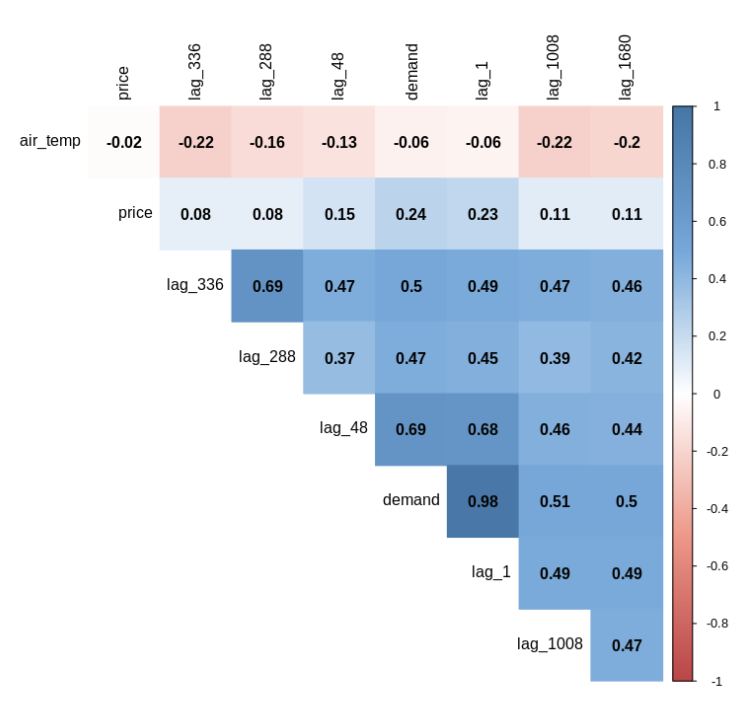
\includegraphics[width=1\linewidth]{correlation}
   \caption{Correlation Heatmap of Select Variables}
   \label{fig:correlation}
\end{minipage}%
\end{figure}


\section{Stationary check and transformation}


\begin{figure}[H]
\centering
\begin{minipage}{.9\textwidth}
  \centering
  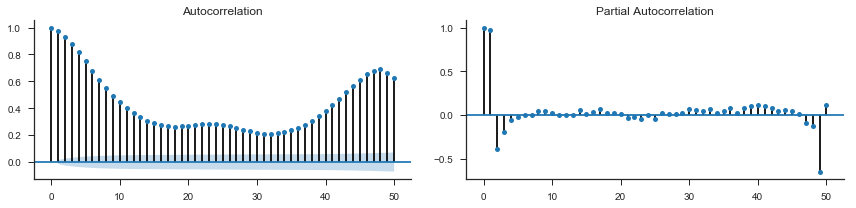
\includegraphics[width=0.95\linewidth]{demand_PCF.png}
   \caption{ACF/PACF plot for demand variable}
   \label{fig:demand_PCF}
\end{minipage}%
\end{figure}

\begin{figure}[H]
\centering
\begin{minipage}{.9\textwidth}
  \centering
  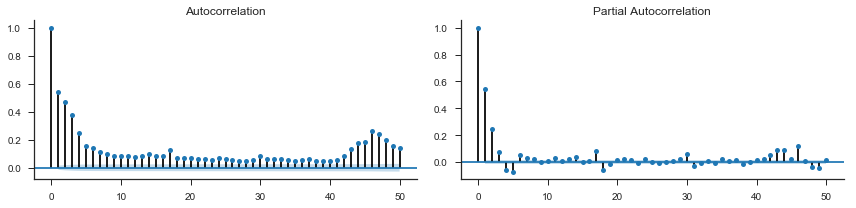
\includegraphics[width=0.95\linewidth]{price_ACF.png}
   \caption{ACF/PACF plot for price variable}
   \label{fig:price_PCF}
\end{minipage}%
\end{figure}

\begin{figure}[H]
\centering
\begin{minipage}{.9\textwidth}
  \centering
  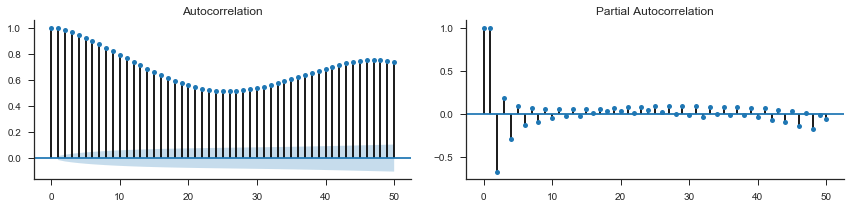
\includegraphics[width=0.95\linewidth]{temp_ACF.png}
   \caption{ACF/PACF plot for temperature variable}
   \label{fig:temp_PCF}
\end{minipage}%
\end{figure}

\section{Auto regressive models}
\label{appendix:auto_regressive_models}

\begin{figure}[H]
\centering
\begin{minipage}{.75\textwidth}
  \centering
  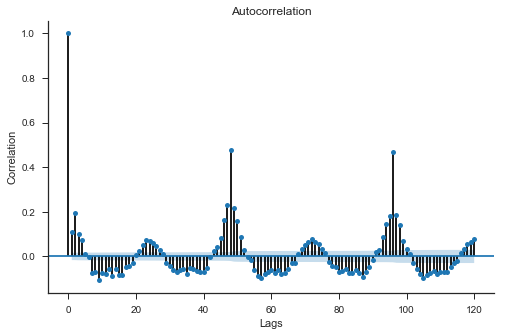
\includegraphics[width=0.95\linewidth]{ACF_AR_1_.png}
   \caption{ACF AR(1)}
   \label{fig:ACF_plot_AR(1)}
\end{minipage}%
\end{figure}

\begin{figure}[H]
\centering
\begin{minipage}{.75\textwidth}
  \centering
  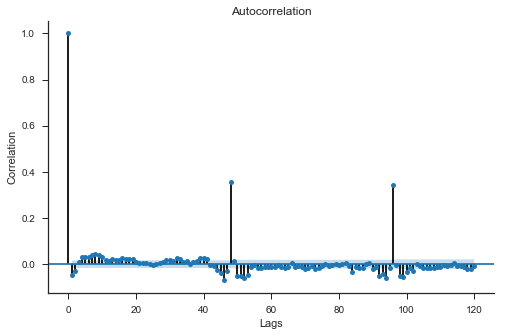
\includegraphics[width=0.95\linewidth]{ACF_AR_48_.png}
   \caption{ACF AR(48)}
   \label{fig:ACF plot for AR(48)}
\end{minipage}%
\end{figure}

\begin{figure}[H]
\centering
\begin{minipage}{.5\textwidth}
  \centering
  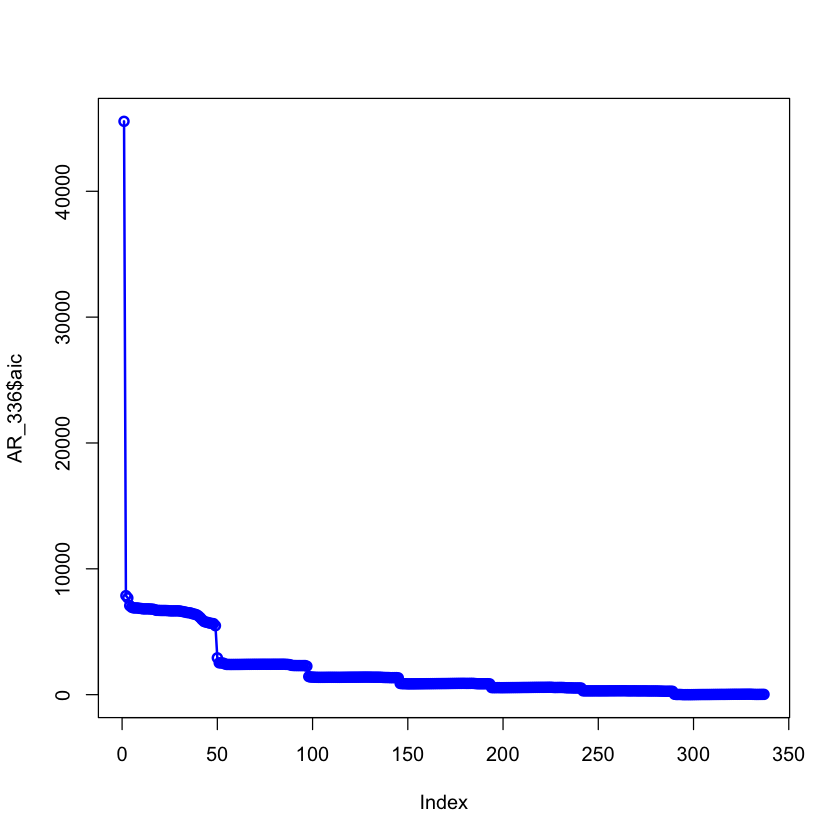
\includegraphics[width=0.95\linewidth]{AR_AIC_train.png}
   \caption{AIC plot by lag number}
   \label{fig:AR_AIC_train}
\end{minipage}%
\end{figure}

\begin{figure}[H]
\centering
\begin{minipage}{.5\textwidth}
  \centering
  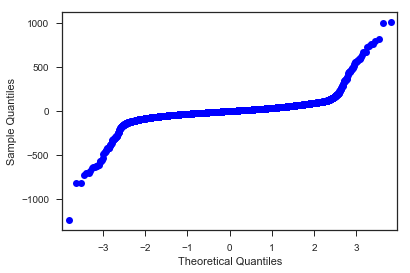
\includegraphics[width=0.95\linewidth]{AR_qq.png}
   \caption{QQ Plot of AR(336)}
   \label{fig:QQ Plot of AR(336)}
\end{minipage}%
\end{figure}

\section{Model Validation}
\label{appendix:model_validation}

This Appendix outlines the further model validation that was completed in this investigation.

\subsection{LASSO}
The best alpha, based on cross-validation on the training data, was $\alpha$ = 0.165. The coefficients are shown in the following plot:

\begin{figure}[H]
\centering
\begin{minipage}{.75\textwidth}
  \centering
  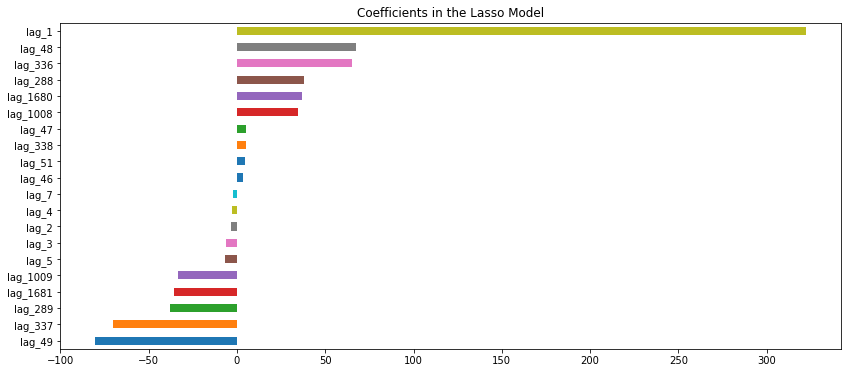
\includegraphics[width=0.95\linewidth]{lasso_co.png}
   \caption{LASSO Coefficient Plot}
   \label{fig:lasso_co_appendix}
\end{minipage}%
\end{figure}

The most important variables were the same as the Ridge case however the LASSO model shrunk 12 coefficients to zero. Hence the LASSO model has reduced variance and is more interpretable compared the ridge model.

\subsection{Elastic net}

The best alpha from our analysis was $\alpha$ = 0.057 with the best $l_1$ ratio = 1.0. This ratio suggests that the elastic net has essentially picked LASSO regression and we expect the LASSO model and elastic net to have similar results. 

\begin{figure}[H]
\centering
\begin{minipage}{.75\textwidth}
  \centering
  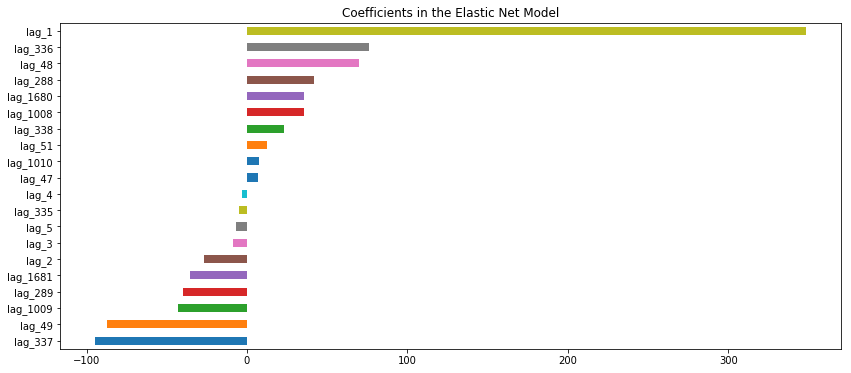
\includegraphics[width=0.95\linewidth]{en_co.png}
   \caption{Elastic Net Coefficient Plot}
   \label{fig:en_co_appendix}
\end{minipage}%
\end{figure}

The elastic net eliminated 8 variables in contrast to LASSO's 12.


\begin{figure}[H]
\centering
\begin{minipage}{.75\textwidth}
  \centering
  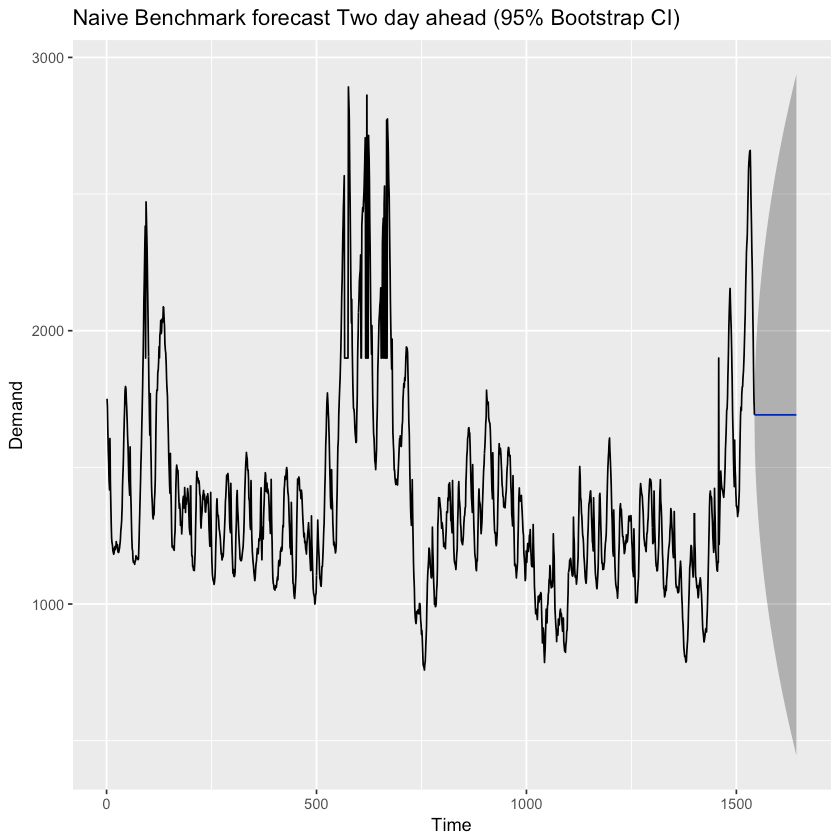
\includegraphics[width=0.95\linewidth]{twodayahead_BS_CI_naive_BM.png}
   \caption{Forecast two days ahead Naive Benchmark 95\% Bootstrap CI}
   \label{fig:twodayahead_BS_CI_naive_BM_appendix}
\end{minipage}%
\end{figure}

\subsection{Neural Network}
\label{appendix:nn_validation_models}

The 3 best neural network models, based on their cross-validation randomised grid search scores, are shown in the following table:

\begin{table}[H]
\centering
\caption{Hyperparameter Optimisation Results}
\label{table:hyperparameter_optimisation_results}
\begin{tabular}{@{}cccc@{}}
\toprule
 & \textbf{NN 1} & \textbf{NN 2} & \textbf{NN 3} \\ \midrule
Layer 1 Neurons & 25 & 25 & 40 \\
Layer 2 Neurons & 25 & 40 & 30 \\
Layer 3 Neurons & 40 & 30 & 30 \\
Weight initilisation & he\_normal & he\_normal & glorot\_normal \\
Epochs & 1200 & 900 & 1200 \\
Batch size & 50 & 10 & 10 \\
Optimisation algorithm & nadam & nadam & adam \\
Dropout & 0.2 & 0.2 & 0.2 \\ 
Max. weight constraint & 3 & 1 & 2 \\ \bottomrule
\end{tabular}
\end{table}

\section{Granger Causality Test Results}

Model 1 is the unrestricted model that includes the Granger-causal terms. Model 2 is the restricted model where the Granger-causal terms are omitted.
The test is a Wald test that assesses whether using the restricted Model 2 in place of Model 1 makes statistical sense (roughly speaking).
\\
\\
H0: No Granger causality
\\
\\
H1: Granger causality
\\
\\
As Pr($<$F)$<$ 0.01, we reject H0 for both price and temperature.

\begin{table}[H]
\centering
\caption{Granger Causality Test: Temperature}
\label{table:granger_temp}
\begin{tabular}{@{}cccc@{}}
\toprule
 \textbf{Res. Df} & \textbf{Df} & \textbf{F} & \textbf{Pr($>$F)} \\ \midrule
17306 & NA & NA & NA \\
17354 & -48 & 6.58 & 1.14e-40\\ \bottomrule
\end{tabular}
\end{table}

\begin{table}[H]
\centering
\caption{Granger Causality Test: Price}
\label{table:granger_price}
\begin{tabular}{@{}cccc@{}}
\toprule
 \textbf{Res. Df} & \textbf{Df} & \textbf{F} & \textbf{Pr($>$F)} \\ \midrule
16442 & NA & NA & NA \\
16778 & -336 & 2.47 & 3.20e-42\\ \bottomrule
\end{tabular}
\end{table}


\section{Neural Network Residuals}
\label{appendix:nn_residuals}

\begin{figure}[H]
\centering
\begin{minipage}{.35\textwidth}
  \centering
  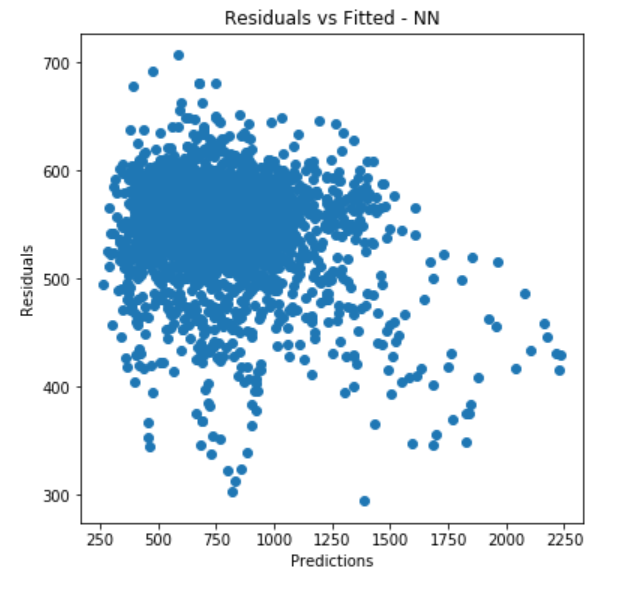
\includegraphics[width=0.95\linewidth]{residuals_fitted_nn_withDummy}
   \caption{Residuals vs. Fitted - NN with Seasonal Dummies}
   \label{fig:residuals_fitted_nn_withDummy}
\end{minipage}%
\end{figure}


\section{One step ahead forecast plots}
\label{appendix:forecast plots}

\begin{figure}[H]
\centering
\begin{minipage}{0.8\textwidth}
  \centering
  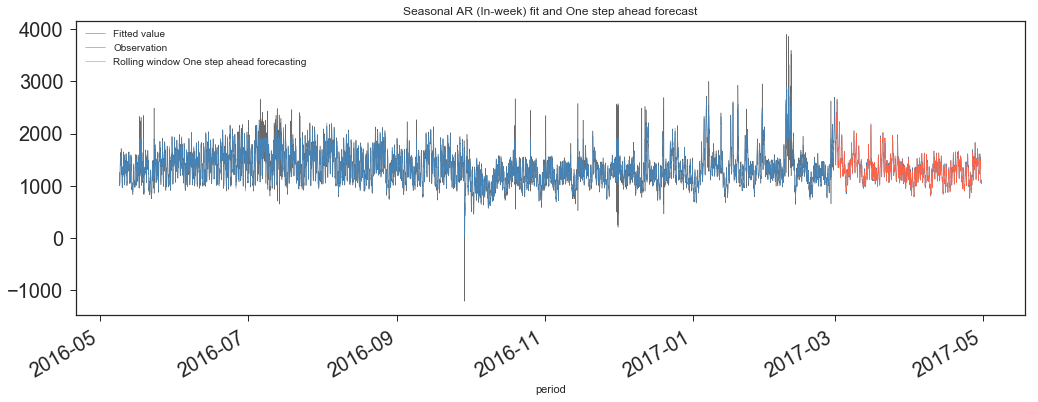
\includegraphics[width=0.95\linewidth]{AR336_plot.png}
   \caption{AR(336) one step ahead forecast}
   \label{fig:AR336_plot}
\end{minipage}%
\end{figure}

\begin{figure}[H]
\centering
\begin{minipage}{0.8\textwidth}
  \centering
  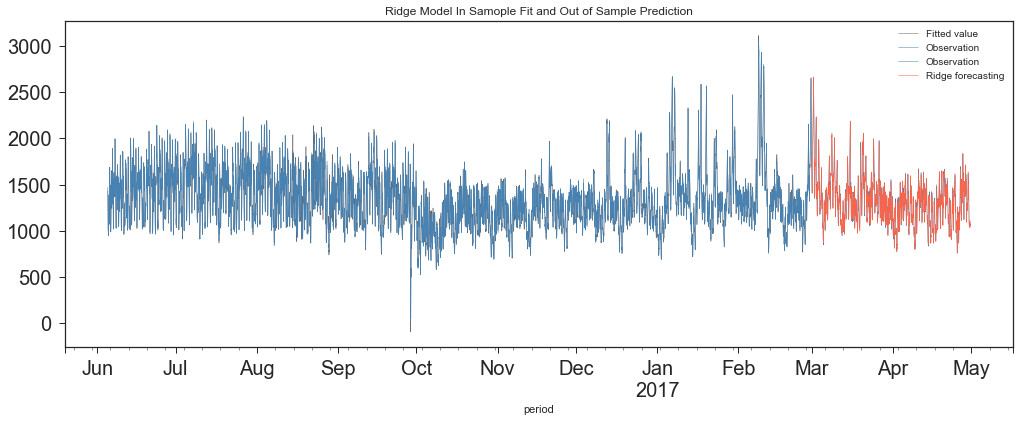
\includegraphics[width=0.95\linewidth]{ridge_plot.png}
   \caption{Ridge Regression one step ahead forecast}
   \label{fig: ridge_plot}
\end{minipage}%
\end{figure}

% Bootstrap residuals
\section{Bootstrap}
\label{appendix:bootstrap}

\subsection{Ridge}
\label{appendix:ridge_bootstrap}

\begin{figure}[H]
\centering
\begin{minipage}{.5\textwidth}
  \centering
  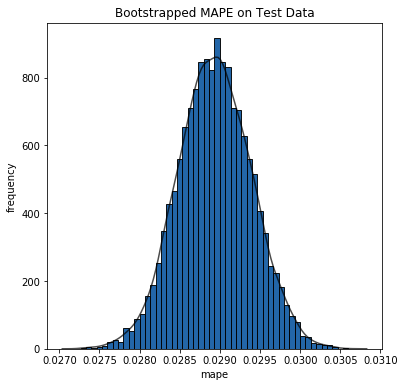
\includegraphics[width=0.95\linewidth]{ridge_mape_boot_dist.png}
   \caption{Ridge: Bootstrap MAPE \\Distribution}
   \label{fig:ridge_mape_boot_dist}
\end{minipage}%
\begin{minipage}{.5\textwidth}
  \centering
  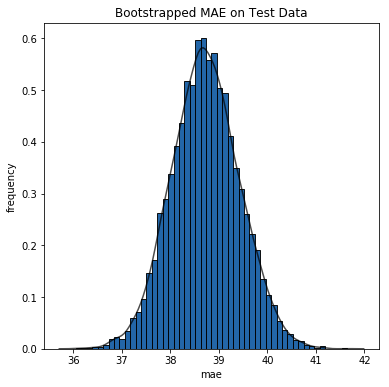
\includegraphics[width=0.95\linewidth]{ridge_mae_boot_dist.png}
   \caption{Ridge: Bootstrap MAE \\Distribution}
   \label{fig:ridge_mae_boot_dist}
\end{minipage}
\end{figure}

\subsection{Neural Network}
\label{appendix:nn_bootstrap}

\begin{figure}[H]
\centering
\begin{minipage}{.5\textwidth}
  \centering
  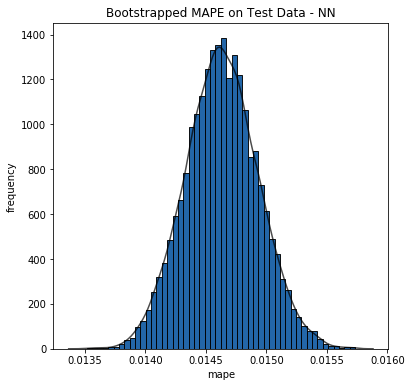
\includegraphics[width=0.95\linewidth]{nn_mape_boot_dist.png}
   \caption{NN: Bootstrap MAPE \\Distribution}
   \label{fig:nn_mape_boot_dist}
\end{minipage}%
\begin{minipage}{.5\textwidth}
  \centering
  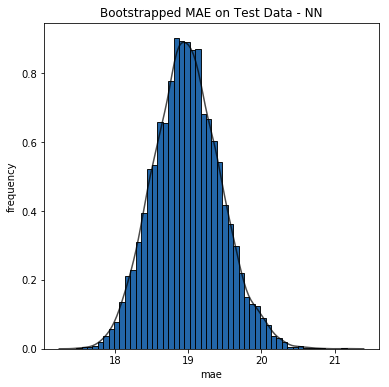
\includegraphics[width=0.95\linewidth]{nn_mae_boot_dist.png}
   \caption{NN: Bootstrap MAE \\Distribution}
   \label{fig:nn_mae_boot_dist}
\end{minipage}
\end{figure}

\subsection{Difference}
\label{appendix:difference_bootstrap}

\begin{figure}[H]
\centering
\begin{minipage}{.5\textwidth}
  \centering
  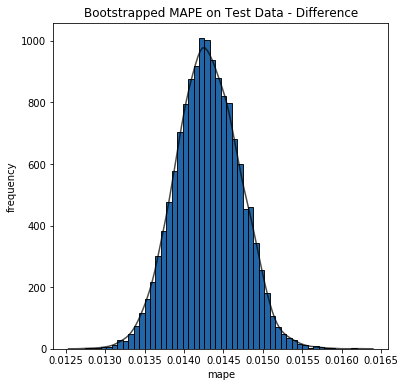
\includegraphics[width=0.95\linewidth]{diff_mape_boot_dist.png}
   \caption{Difference: Bootstrap MAPE \\Distribution}
   \label{fig:diff_mape_boot_dist}
\end{minipage}%
\begin{minipage}{.5\textwidth}
  \centering
  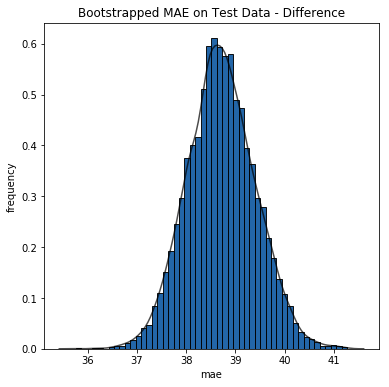
\includegraphics[width=0.95\linewidth]{diff_mae_boot_dist.png}
   \caption{Difference: Bootstrap MAE \\Distribution}
   \label{fig:diff_mae_boot_dist}
\end{minipage}
\end{figure}

\subsection{Diagnostics}
\label{appendix:diagnostics}

\begin{figure}[H]
\centering
\begin{minipage}{.5\textwidth}
  \centering
  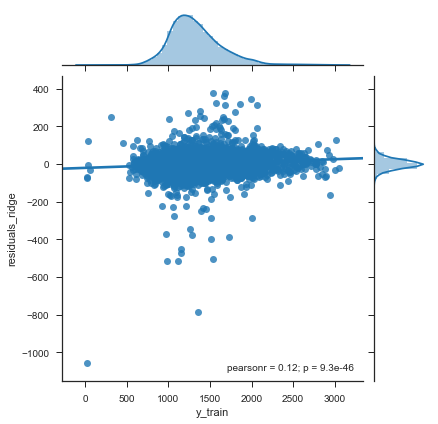
\includegraphics[width=0.95\linewidth]{ridge_residual.png}
   \caption{Residuals vs. Fitted - Ridge Regression}
   \label{fig:residuals_fitted_ridge_appendix}
\end{minipage}%
\end{figure}

\setlength{\parskip}{1em}
\end{document}


